\documentclass[]{article}
\usepackage{lmodern}
\usepackage{amssymb,amsmath}
\usepackage{ifxetex,ifluatex}
\usepackage{fixltx2e} % provides \textsubscript
\ifnum 0\ifxetex 1\fi\ifluatex 1\fi=0 % if pdftex
  \usepackage[T1]{fontenc}
  \usepackage[utf8]{inputenc}
\else % if luatex or xelatex
  \ifxetex
    \usepackage{mathspec}
  \else
    \usepackage{fontspec}
  \fi
  \defaultfontfeatures{Ligatures=TeX,Scale=MatchLowercase}
\fi
% use upquote if available, for straight quotes in verbatim environments
\IfFileExists{upquote.sty}{\usepackage{upquote}}{}
% use microtype if available
\IfFileExists{microtype.sty}{%
\usepackage{microtype}
\UseMicrotypeSet[protrusion]{basicmath} % disable protrusion for tt fonts
}{}
\usepackage[margin=1in]{geometry}
\usepackage{hyperref}
\hypersetup{unicode=true,
            pdftitle={Exerciții de seminar 2},
            pdfborder={0 0 0},
            breaklinks=true}
\urlstyle{same}  % don't use monospace font for urls
\usepackage{natbib}
\bibliographystyle{plainnat}
\usepackage{graphicx,grffile}
\makeatletter
\def\maxwidth{\ifdim\Gin@nat@width>\linewidth\linewidth\else\Gin@nat@width\fi}
\def\maxheight{\ifdim\Gin@nat@height>\textheight\textheight\else\Gin@nat@height\fi}
\makeatother
% Scale images if necessary, so that they will not overflow the page
% margins by default, and it is still possible to overwrite the defaults
% using explicit options in \includegraphics[width, height, ...]{}
\setkeys{Gin}{width=\maxwidth,height=\maxheight,keepaspectratio}
\IfFileExists{parskip.sty}{%
\usepackage{parskip}
}{% else
\setlength{\parindent}{0pt}
\setlength{\parskip}{6pt plus 2pt minus 1pt}
}
\setlength{\emergencystretch}{3em}  % prevent overfull lines
\providecommand{\tightlist}{%
  \setlength{\itemsep}{0pt}\setlength{\parskip}{0pt}}
\setcounter{secnumdepth}{5}
% Redefines (sub)paragraphs to behave more like sections
\ifx\paragraph\undefined\else
\let\oldparagraph\paragraph
\renewcommand{\paragraph}[1]{\oldparagraph{#1}\mbox{}}
\fi
\ifx\subparagraph\undefined\else
\let\oldsubparagraph\subparagraph
\renewcommand{\subparagraph}[1]{\oldsubparagraph{#1}\mbox{}}
\fi

%%% Use protect on footnotes to avoid problems with footnotes in titles
\let\rmarkdownfootnote\footnote%
\def\footnote{\protect\rmarkdownfootnote}

%%% Change title format to be more compact
\usepackage{titling}

% Create subtitle command for use in maketitle
\newcommand{\subtitle}[1]{
  \posttitle{
    \begin{center}\large#1\end{center}
    }
}

\setlength{\droptitle}{-2em}
  \title{Exerciții de seminar 2}
  \pretitle{\vspace{\droptitle}\centering\huge}
  \posttitle{\par}
\subtitle{Regresie}
  \author{}
  \preauthor{}\postauthor{}
  \date{}
  \predate{}\postdate{}

\usepackage{booktabs}
\usepackage{longtable}
\usepackage{framed,color}
\definecolor{shadecolor}{RGB}{248, 248, 248}
%\definecolor{shadecolor1}{RGB}{216,225,235}
%\definecolor{framecolor}{RGB}{108,123,13}

%\definecolor{shadecolor}{RGB}{226, 255, 241}
\definecolor{shadecolor1}{RGB}{217,225,199}
\definecolor{framecolor}{RGB}{60,179,113}

\ifxetex
  \usepackage{letltxmacro}
  \setlength{\XeTeXLinkMargin}{1pt}
  \LetLtxMacro\SavedIncludeGraphics\includegraphics
  \def\includegraphics#1#{% #1 catches optional stuff (star/opt. arg.)
    \IncludeGraphicsAux{#1}%
  }%
  \newcommand*{\IncludeGraphicsAux}[2]{%
    \XeTeXLinkBox{%
      \SavedIncludeGraphics#1{#2}%
    }%
  }%
\fi

\newenvironment{frshaded*}{%
  \def\FrameCommand{\fboxrule=\FrameRule\fboxsep=\FrameSep \fcolorbox{framecolor}{shadecolor1}}%
  \MakeFramed {\advance\hsize-\width \FrameRestore}}%
{\endMakeFramed}

\newenvironment{rmdblock}[1]
  {\begin{frshaded*}
  \begin{itemize}
  \renewcommand{\labelitemi}{
    \raisebox{-.7\height}[0pt][0pt]{
      {\setkeys{Gin}{width=2em,keepaspectratio}\includegraphics{images/icons/#1}}
    }
  }
  \item
  }
  {
  \end{itemize}
  \end{frshaded*}
  }

\newenvironment{rmdcaution}
  {\begin{rmdblock}{caution}}
  {\end{rmdblock}}
% \newenvironment{rmdinsight}
%   {\begin{rmdblock}{insight}}
%   {\end{rmdblock}}
\newenvironment{rmdexercise}
  {\begin{rmdblock}{exercise}}
  {\end{rmdblock}}
\newenvironment{rmdtip}
  {\begin{rmdblock}{tip}}
  {\end{rmdblock}}


%%%%%%%%%%%%%%%%%%%%%%%%%%%%%%%%%%%%%%%%%%%%%%%%%%%%%%%%%%%%%%%%%%%%%%%%%%%%%%%%%%%%%%%%%%%%%%%%%%%%%%%%%%%%%%%%%%%%%
%%%%%%%%%%% For insight block %%%%%%%%%%%%%%%%%%%%%%%%%%
\definecolor{shadecolor_insight}{RGB}{223,240,216}
\definecolor{framecolor_insight}{RGB}{136,193,137}

%\definecolor{shadecolor_insight}{RGB}{217,225,199}
%\definecolor{framecolor_insight}{RGB}{60,179,113}

\newenvironment{frshaded_insight*}{%
  \def\FrameCommand{\fboxrule=\FrameRule\fboxsep=\FrameSep \fcolorbox{framecolor_insight}{shadecolor_insight}}%
  \MakeFramed {\advance\hsize-\width \FrameRestore}}%
{\endMakeFramed}

\newenvironment{rmdblock_insight}[1]
  {\begin{frshaded_insight*}
  \begin{itemize}
  \renewcommand{\labelitemi}{
    \raisebox{-.7\height}[0pt][0pt]{
      {\setkeys{Gin}{width=2em,keepaspectratio}\includegraphics{images/icons/#1}}
    }
  }
  \item
  }
  {
  \end{itemize}
  \end{frshaded_insight*}
  }

\newenvironment{rmdinsight}
  {\begin{rmdblock_insight}{insight}}
  {\end{rmdblock_insight}}

%%%%%%%%%%%%%%%%%%%%%%%%%%%%%%%%%%%%%%%%%%%%%%%%%%%%%%%%%%%%%%%%%%%%%%%%%%%%%%%%%%%%%%%%%%%%%%%%%%%%%%%%%%%%%%%%%%%%%
\usepackage{subfigure}
\usepackage{booktabs}
\usepackage{slashbox}
\usepackage{color}
%%%%%%%%%%%%%%%%%%%%%%%%%%%%%%%%%%%%%%%%%
\definecolor{linkcol}{rgb}{0,0,0.4}
\definecolor{citecol}{rgb}{0.5,0,0}

% Change this to change the informations included in the pdf file
% \usepackage[pagebackref]{hyperref}
% \usepackage[verbose]{backref}
\usepackage[hyperpageref]{backref}
% \backrefsetup{verbose=false}
% \PassOptionsToPackage{pagebackref}{hyperref}
% See hyperref documentation for information on those parameters

\hypersetup
{
bookmarksopen=true,
pdftitle="Curs Instrumente Statistice pentru Finante",
pdfauthor="Alexandru Amarioarei",
pdfsubject="Laboratoare Instrumente Statistice pentru Finante", %subject of the document
pdfmenubar=true, %menubar shown
pdfhighlight=/O, %effect of clicking on a link
colorlinks=true, %couleurs sur les liens hypertextes
pdfpagemode=None, %aucun mode de page
pdfpagelayout=SinglePage, %ouverture en simple page
pdffitwindow=true, %pages ouvertes entierement dans toute la fenetre
linkcolor=linkcol, %couleur des liens hypertextes internes
citecolor=citecol, %couleur des liens pour les citations
urlcolor=linkcol %couleur des liens pour les url
}


% set the back references
\renewcommand*{\backref}[1]{}
\renewcommand*{\backreftwosep}{ și~} % inserted between entries 
                              % in a list of two entries, 
                              % default is " and~".
\renewcommand*{\backreflastsep}{ și~} % inserted between the last 
                               % two entries of a list with more
                               % than two entries, default is ", and~".
\renewcommand*{\backrefalt}[4]{%
    \ifcase #1 (Necitat.)%
    \or        (Citat la pagina~#2.)%
    \else      (Citat la paginile~#2.)%
    \fi}

%%%%%%%%%%%%%%%%%%%%%%%%%%%%%%%%%%%%%%%%%%%%%%%%%%%%%%%%%%%%%%%%%%%%%%%%%%%%%%%%%%%%%%%%%%%%%%%%%%%%%%%%%%%%%%%%%%%%%
%CITEVA DEFINITII
\def\om{\omega}
\def\Om{\Omega}
\def\et{\eta}
\def\td{\tilde{\delta}}
\def\m{{\mu}}
\def\n{{\nu}}
\def\k{{\kappa}}
\def\l{{\lambda}}
\def\L{{\Lambda}}
\def\g{{\gamma}}
\def\a{{\alpha}}
\def\e{{\varepsilon}}
\def\b{{\beta}}
\def\G{{\Gamma}}
\def\d{{\delta}}
\def\D{{\Delta}}
\def\t{{\theta}}
\def\s{{\sigma}}
\def\S{{\Sigma}}
\def\z{{\zeta}}
\def\qed{\hfill\Box}
\def\ds{\displaystyle}
\def\mc{\mathcal}
%%%%%%%%%%%%%%%%%%%%%%%%%%%%%%%%%%%%%%%%%%%%%%%%%%%%%%%%%%%%%%%%%%%%%%%%%%%%%%%%%%%%%%%%%%%%%%%%%%%%%%%%%%%%%%%%%%%%%%
\def\1{{\mathbf 1}}
\def\CC{{\mathbb C}}
\def\VV{{\mathbb V}}
\def\RR{{\mathbb R}}
\def\QQ{{\mathbb Q}}
\def\ZZ{{\mathbb Z}}
\def\PP{{\mathbb P}}
\def\EE{{\mathbb E}}
\def\NN{{\mathbb N}}
\def\FF{{\mathbb F}}
%\def\SS{{\mathbb S}}
\def\MA{{\mathcal A}}
\def\MO{{\mathcal O}}
\def\MF{{\mathcal F}}
\def\ME{{\mathcal E}}
\def\MR{{\mathcal R}}
\def\MB{{\mathcal B}}
\def\MM{{\mathcal M}}
\def\MN{{\mathcal N}}
\def\MU{{\mathcal U}}
\def\MP{{\mathcal P}}
\def\MS{{\mathcal S}}
\def\MBS{{\mathbf S}}
\def\MX{{\bm{ \mathscr X}}}

% independent sign
\newcommand\independent{\protect\mathpalette{\protect\independenT}{\perp}}
\def\independenT#1#2{\mathrel{\rlap{$#1#2$}\mkern2mu{#1#2}}}

\renewcommand\tablename{Tab.}
\renewcommand{\figurename}{Fig.}
\renewcommand\refname{Referințe}

%%%%%%%%%%%%%%%%%%%%%%%%%%%%%%%%%%%%%%%%%%%%%%%%%%%%%%%%%%%%%%%%%%%%%%%%%%%%%%%%%%%%%%%%%%%%%%%%%%%%%%%%%%%%%%%%%%%%%
%Header and Footer
\usepackage{fancyhdr}

\pagestyle{fancy}
\fancyhf{}
\rhead{Universitatea din Bucure\c sti\\ Facultatea de Matematic\u a \c si Informatic\u a}
\lhead{\textit{Curs}: Instrumente Statistice pentru Finan\c te\\ \textit{Instructor}: A. Am\u arioarei}
\rfoot{Pagina \thepage}
\lfoot{Grupa: 403}
%%%%%%%%%%%%%%%%%%%%%%%%%%%%%%%%%%%%%%%
\usepackage{booktabs}
\usepackage{longtable}
\usepackage{array}
\usepackage{multirow}
\usepackage[table]{xcolor}
\usepackage{wrapfig}
\usepackage{float}
\usepackage{colortbl}
\usepackage{pdflscape}
\usepackage{tabu}
\usepackage{threeparttable}
\usepackage{threeparttablex}
\usepackage[normalem]{ulem}
\usepackage{makecell}

\begin{document}
\maketitle

%%%%%%%%%%%%%%%%%%%%%%%%
\thispagestyle{fancy}

Obiectivul acestui seminar este de a prezenta câteva exerciții de
regresie liniară.

\section{Regresie liniară simplă}\label{regresie-liniara-simpla}

\subsection{Interpretări geometrice}\label{interpretari-geometrice}

În această secțiune încercăm să abordăm problema de regresie liniară
simplă într-un context geometric. Din punct de vedere vectorial dispunem
de doi vectori: vectorul \(X = (x_1, x_2, \ldots, x_n)^\intercal\) a
celor \(n\) observații ale variabilei explicative și vectorul
\(Y = (y_1, y_2, \ldots, y_n)^\intercal\) compus din cele \(n\)
observații ale variabilei răspuns, pe care vrem să o explicăm. Cei doi
vectori aparțin spațiului \(\mathbb{R}^n\).

Fie \(\mathbf{1} = (1,1,\ldots,1)^\intercal\in\mathbb{R}^n\) și
\(\mathcal{M}(X)\) subspațiul liniar din \(\mathbb{R}^n\) de dimensiune
\(2\) generat de vectorii \(\{\mathbf{1}, X\}\) (acești vectori nu sunt
coliniari deoarece \(X\) conține cel puțin două elemente distincte).
Notăm cu \(\hat Y\) proiecția ortogonală a lui \(Y\) pe subspațiul
\(\mathcal{M}(X)\) și cum \(\{\mathbf{1}, X\}\) formează o bază în
\(\mathcal{M}(X)\) deducem că există
\(\hat\beta_0, \hat\beta_1\in \mathbb{R}\) astfel ca
\(\hat Y = \hat\beta_0\mathbf{1} + \hat\beta_1 X\). Cum, din definiția
priecției ortogonale, \(\hat Y\) este unicul vector din
\(\mathcal{M}(X)\) care minimizează distanța euclidiană (deci și
pătratul ei)

\[
\left\lVert Y - \hat Y \right\rVert = \sum_{i = 1}^{n}[y_i - (\hat\beta_0 + \hat \beta_1 x_i)]^2
\]

deducem că \(\hat\beta_0, \hat\beta_1\) coincid cu valorile obținute
prin metoda celor mai mici pătrate. Astfel coeficienții \(\hat\beta_0\)
și \(\hat\beta_1\) se reprezintă coordonatele proiecției ortogonale a
lui \(Y\) pe subspațiul generat de vectorii \(\{\mathbf{1}, X\}\) (a se
vedea figura de mai jos).

\begin{center}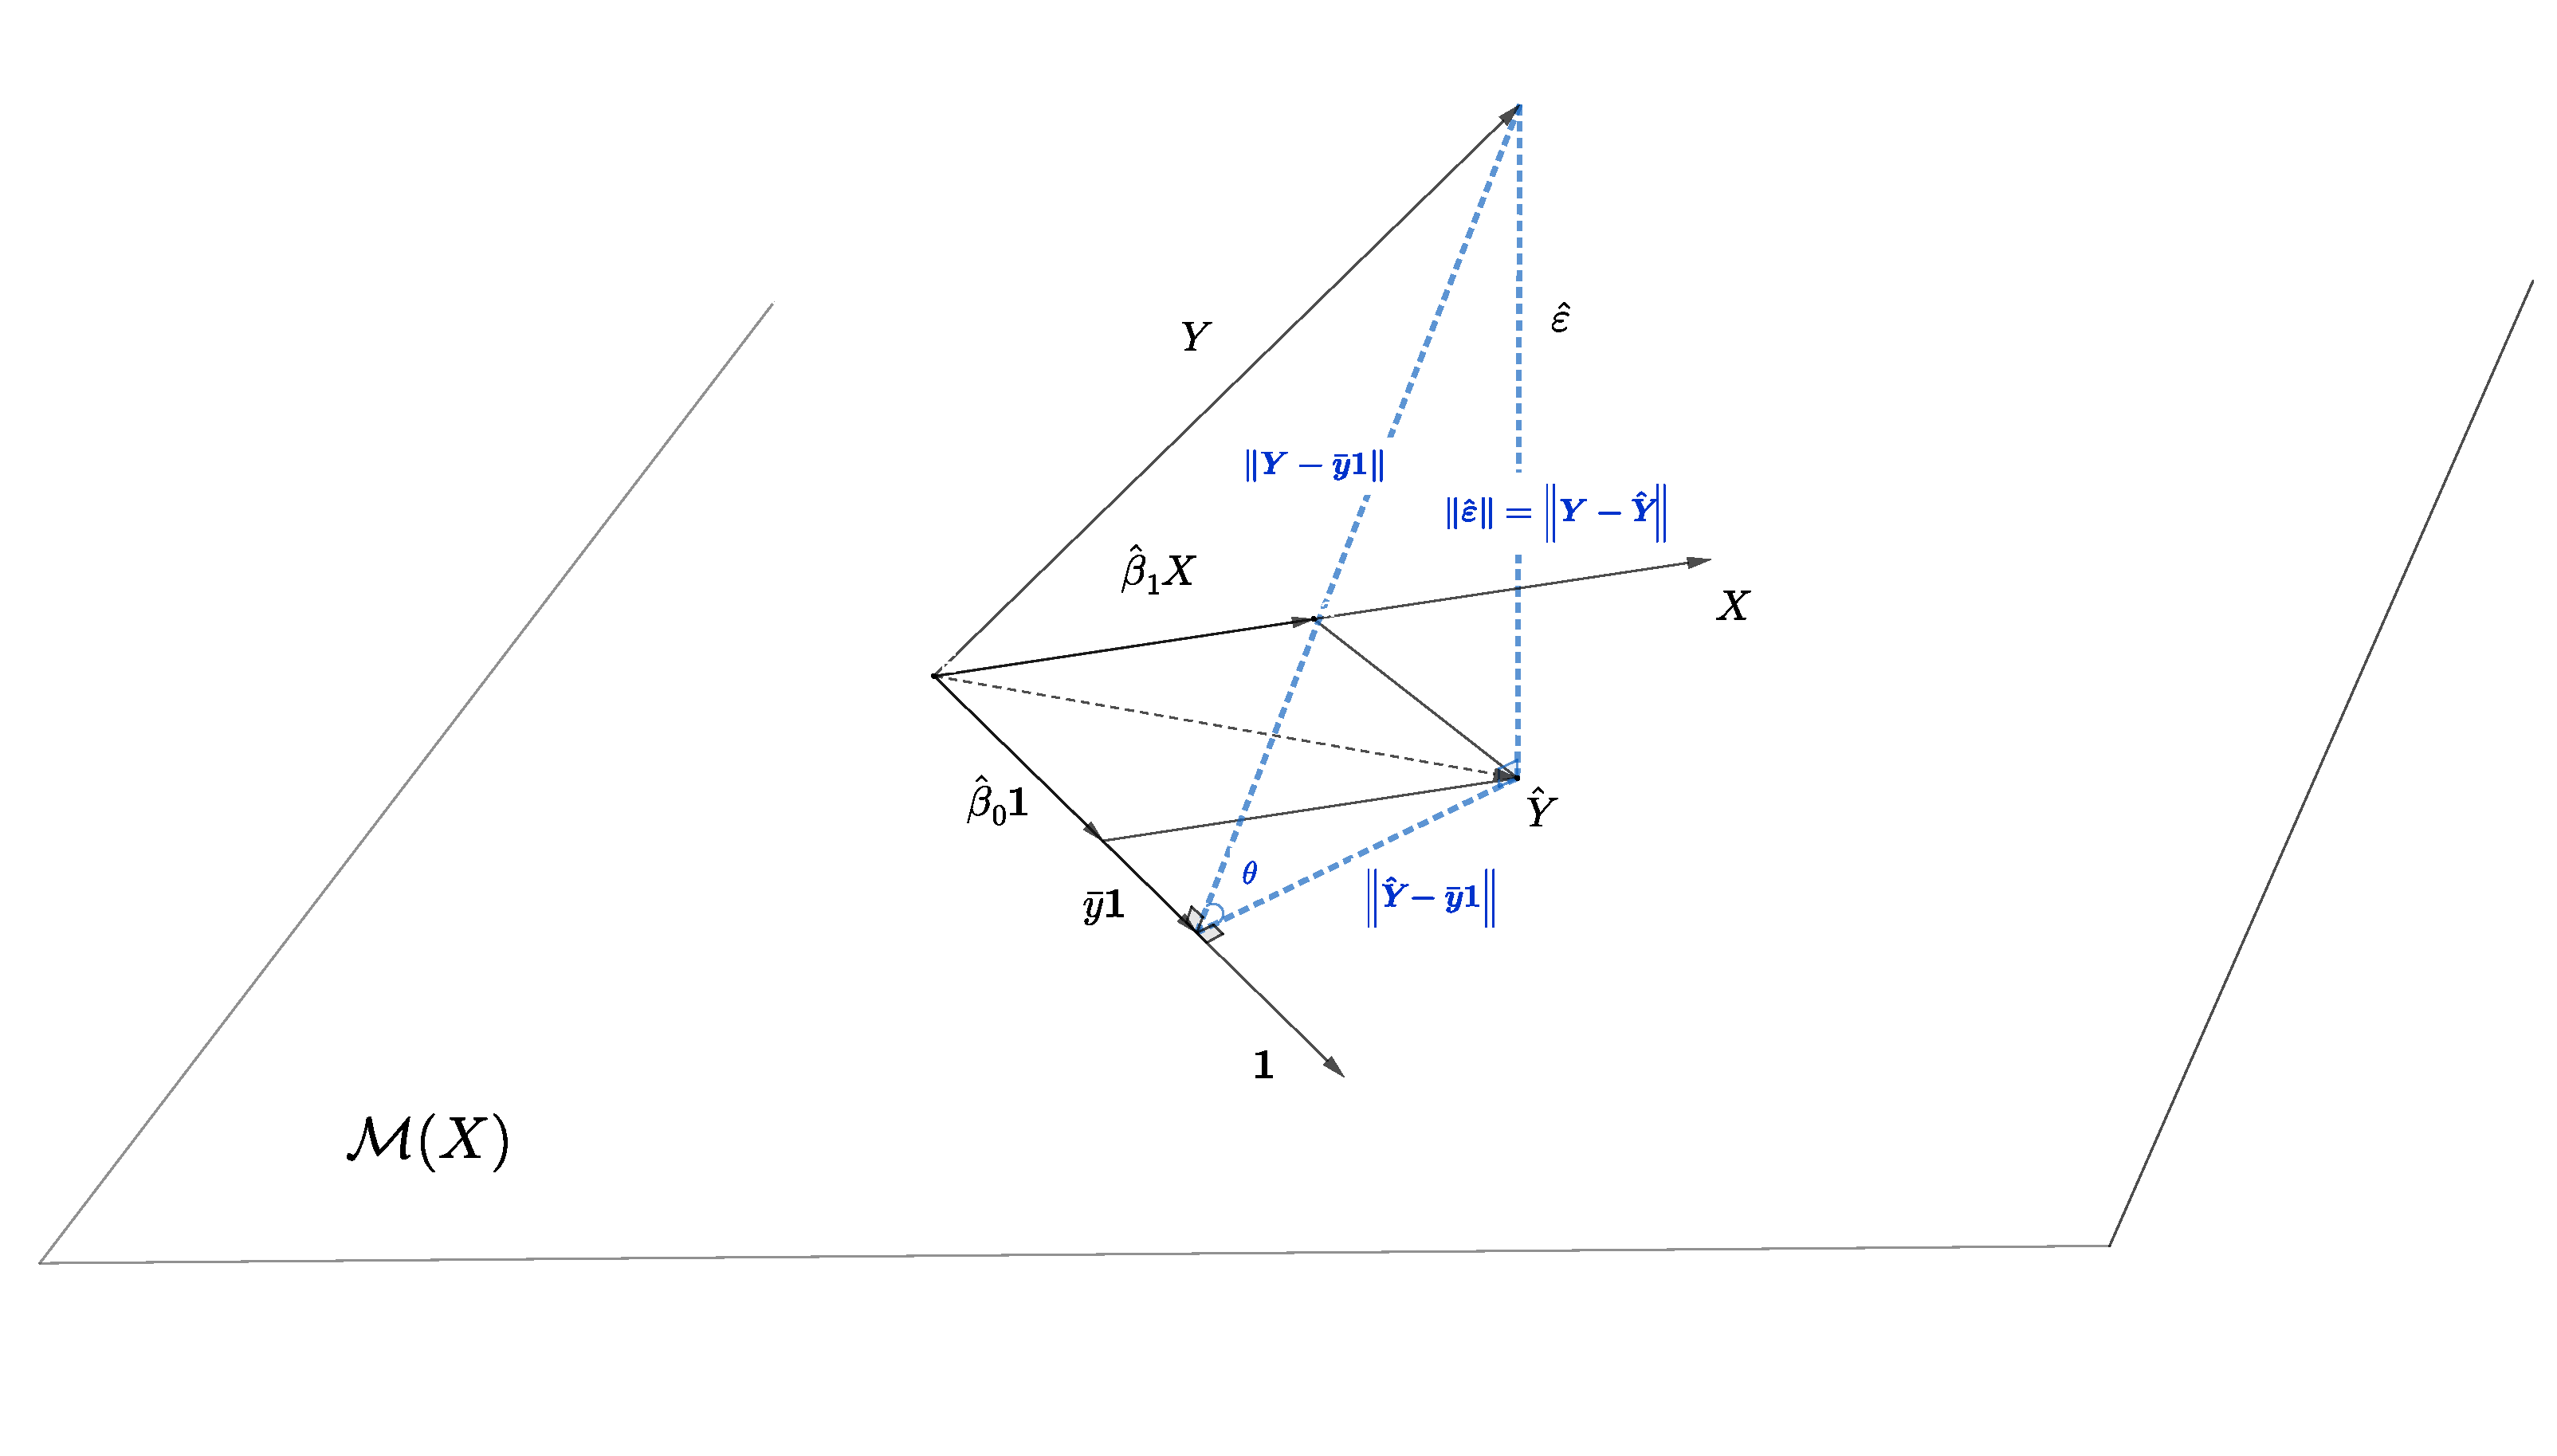
\includegraphics[width=0.8\linewidth]{images/sem2/reg_int_geom5} \end{center}

Observăm că, în general, vectorii \(\{\mathbf{1}, X\}\) nu formează o
bază ortogonală în \(\mathcal{M}(X)\) (cu excepția cazului în care
\(\langle \mathbf{1}, X\rangle = n\bar x = 0\)) prin urmare
\(\hat\beta_0\mathbf{1}\) nu este proiecția ortogonală a lui \(Y\) pe
\(\mathbf{1}\) (aceasta este
\(\frac{\langle Y, \mathbf{1}\rangle}{\lVert \mathbf{1}\rVert^2}\mathbf{1} = \bar y\mathbf{1}\))
iar \(\hat\beta_1 X\) nu este proiecția ortogonală a lui \(Y\) pe \(X\)
(aceasta fiind \(\frac{\langle Y, X\rangle}{\lVert X\rVert^2}X\)).

Fie
\(\hat\varepsilon = Y - \hat Y = (\hat\varepsilon_1, \hat\varepsilon_2, \ldots, \hat\varepsilon_n)^\intercal\)
vectorul valorilor reziduale. Aplicând Teorema lui Pitagora (în
triunghiul albastru) rezultă (descompunerea ANOVA pentru regresie) că

\begin{align*}
  \left\lVert Y - \bar y \mathbf{1}\right\rVert^2 &= \left\lVert \hat Y - \bar y \mathbf{1}\right\rVert^2 + \left\lVert \underbrace{\hat\varepsilon}_{Y - \hat Y}\right\rVert^2\\
  \sum_{i = 1}^{n}(y_i - \bar y)^2 &= \sum_{i = 1}^{n}(\hat y_i - \bar y)^2 + \sum_{i = 1}^{n}(\underbrace{\hat\varepsilon_i}_{y_i - \hat y_i})^2\\
  SS_T &= SS_{reg} + RSS
\end{align*}

Din definiția coeficientului de determinare \(R^2\) avem că

\[
R^2 = \frac{SS_{reg}}{SS_T} = \frac{\left\lVert \hat Y - \bar y \mathbf{1}\right\rVert^2}{\left\lVert Y - \bar y \mathbf{1}\right\rVert^2} = 1 - \frac{\left\lVert \hat \varepsilon\right\rVert^2}{\left\lVert Y - \bar y \mathbf{1}\right\rVert^2}
\]

și conform figurii de mai sus \(R^2 = \cos^2(\theta)\). Prin urmare dacă
\(R^2 = 1\), atunci \(\theta = 0\) și \(Y\in\mathcal{M}(X)\), deci
\(y_i = \beta_0 + \beta_1 x_i\), \(i\in\{1,2,\ldots,n\}\) (punctele
eșantionului sunt perfect aliniate) iar dacă \(R^2 = 0\), deducem că
\(\sum_{i = 1}^{n}(\hat y_i - \bar y)^2 = 0\), deci
\(\hat y_i = \bar y\) (modelul liniar nu este adaptat în acest caz, nu
putem explica mai bine decât media).

\subsection{Metoada celor mai mici
pătrate}\label{metoada-celor-mai-mici-patrate}

\begin{rmdexercise}
Arătați că estimatorii obținuți prin metoda celor mai mici pătrate,
\(\hat\beta_0\) și \(\hat\beta_1\), sunt estimatori nedeplasați.
\end{rmdexercise}

Coeficienții \(\hat\beta_0\) și \(\hat\beta_1\) obținuți prin metoda
celor mai mici pătrate sunt dați de
\(\hat\beta_0 = \bar y - \hat\beta_1 \bar x\) și
\(\hat\beta_1 = \frac{\sum_{i = 1}^{n}(x_i - \bar x)(y_i - \bar y)}{\sum_{i = 1}^{n}(x_i - \bar x)^2}\)
(aceștia sunt variabile aleatoare deoarece sunt funcții de \(Y_i\) care
sunt variabile aleatoare). Înlocuind în expresia lui \(\hat\beta_1\) pe
\(y_i\) cu \(\beta_0+\beta_1 x_i + \varepsilon_i\) avem

\begin{align*}
\hat\beta_1 &= \frac{\sum_{i = 1}^{n}(x_i - \bar x)(y_i - \bar y)}{\sum_{i = 1}^{n}(x_i - \bar x)^2} = \frac{\sum_{i = 1}^{n}(x_i - \bar x)y_i}{\sum_{i = 1}^{n}(x_i - \bar x)^2} = \frac{\sum_{i = 1}^{n}(x_i - \bar x)(\beta_0+\beta_1 x_i + \varepsilon_i)}{\sum_{i = 1}^{n}(x_i - \bar x)^2}\\
  &= \frac{\beta_0\overbrace{\sum_{i = 1}^{n}(x_i - \bar x)}^{ = 0} + \beta_1 \sum_{i = 1}^{n}(x_i - \bar x)x_i + \sum_{i = 1}^{n}(x_i - \bar x)\varepsilon_i}{\sum_{i = 1}^{n}(x_i - \bar x)^2} = \frac{\beta_1 \sum_{i = 1}^{n}(x_i - \bar x)^2 + \sum_{i = 1}^{n}(x_i - \bar x)\varepsilon_i}{\sum_{i = 1}^{n}(x_i - \bar x)^2}\\
  &= \beta_1 + \frac{\sum_{i = 1}^{n}(x_i - \bar x)\varepsilon_i}{\sum_{i = 1}^{n}(x_i - \bar x)^2}.
\end{align*}

Conform ipotezei modelului de regresie liniară simplă,
\(\mathbb{E}[\varepsilon_i] = 0\), prin urmare
\(\mathbb{E}[\hat\beta_1] = \beta_1\) ceea ce arată că \(\hat\beta_1\)
este un estimator nedeplasat pentru \(\beta_1\).

În mod similar,

\[
\mathbb{E}[\hat\beta_0] = \mathbb{E}[\bar y] - \bar x\mathbb{E}[\hat\beta_1] = \beta_0 + \bar x\beta_1 - \bar x\beta_1 = \beta_0
\] ceea ce arată că \(\hat\beta_0\) este un estimator nedeplasat pentru
\(\beta_0\).

\begin{rmdexercise}
Calculați matricea de varianță-covarianță a estimatorilor
\(\hat\beta_0\) și \(\hat\beta_1\).
\end{rmdexercise}

Notăm cu
\(W = \begin{pmatrix}Var(\hat \beta_0) & Cov(\hat \beta_0, \hat \beta_1)\\ Cov(\hat \beta_0, \hat \beta_1) & Var(\hat \beta_1)\end{pmatrix}\)
matricea de varianță-covarianță a estimatorilor \(\hat\beta_0\) și
\(\hat\beta_1\).

Avem, folosind expresia lui \(\hat\beta_1\) determinată la punctul
anterior și homoscedasticitatea și necorelarea erorilor
\(Cov(\varepsilon_i, \varepsilon_j) = \delta_{ij}\sigma^2\), că

\begin{align*}
  Var(\hat \beta_1) &= Var\left(\beta_1 + \frac{\sum_{i = 1}^{n}(x_i - \bar x)\varepsilon_i}{\sum_{i = 1}^{n}(x_i - \bar x)^2}\right) = Var\left(\frac{\sum_{i = 1}^{n}(x_i - \bar x)\varepsilon_i}{\sum_{i = 1}^{n}(x_i - \bar x)^2}\right)\\
  &= \frac{Var\left(\sum_{i = 1}^{n}(x_i - \bar x)\varepsilon_i\right)}{\left[\sum_{i = 1}^{n}(x_i - \bar x)^2\right]^2} = \frac{\sum_{i,j}(x_i - \bar x)(x_j - \bar x)Cov(\varepsilon_i, \varepsilon_j)}{\left[\sum_{i = 1}^{n}(x_i - \bar x)^2\right]^2}\\
  &= \frac{\sum_{i = 1}^{n}(x_i - \bar x)^2\sigma^2}{\left[\sum_{i = 1}^{n}(x_i - \bar x)^2\right]^2} = \frac{\sigma^2}{\sum_{i = 1}^{n}(x_i - \bar x)^2}.
\end{align*}

Din expresia \(Var(\hat \beta_1)\) observăm că dacă \(\sigma^2\) este
mică (cu alte cuvinte \(y_i\) sunt aproape de dreapta de regresie)
atunci estimarea este mai precisă. De asemenea, se constată că pe măsură
ce valorile \(x_i\) sunt mai dispersate în jurul valorii medii
\(\bar x\) estimarea coeficientului \(\hat \beta_1\) este mai precisă
(\(Var(\hat \beta_1)\) este mai mică). Acest fenomen se poate observa și
în figura de mai jos în care am generat \(100\) de valori aleatoare
\(X\) și \(100\) de valori pentru \(Y\) după modelul

\[
  y = 1 + 2 x + \varepsilon
\] cu \(\varepsilon\sim \mathcal{N}(0, \sigma^2)\). Dreapta roșie
descrie adevărata relație \(f(x) = 1 + 2x\) în populație iar dreapta
albastră reprezintă dreapta de regresie calculată cu ajutorul metodei
celor mai mici pătrate (OLS). Dreptele albastru deschis au fost generate
tot cu ajutorul metodei celor mai mici pătrate atunci când variem
\(\sigma^2\) (în figura din stânga) și respectiv pe \(x_i\) în jurul lui
\(\bar x\) (în figura din dreapta).

\begin{center}\includegraphics[width=0.8\linewidth]{Sem_2_files/figure-latex/unnamed-chunk-5-1} \end{center}

Pentru a determina \(Var(\hat \beta_0)\), vom folosi relația
\(\hat \beta_0 = \bar y - \hat \beta_1 \bar x\) ceea ce conduce la

\begin{align*}
Var(\hat \beta_0) &= Var(\bar y - \hat \beta_1 \bar x) = Var(\bar y) - 2Cov(\bar y, \hat \beta_1 \bar x) + Var(\hat \beta_1 \bar x)\\
&= Var\left(\frac{1}{n}\sum_{i = 1}^{n}y_i\right) - 2\bar x Cov(\bar y, \hat \beta_1) + \bar x^2 Var(\hat \beta_1)\\
&= \frac{\sigma^2}{n} + \bar x^2 \frac{\sigma^2}{\sum_{i = 1}^{n}(x_i - \bar x)^2} - 2\bar x Cov(\bar y, \hat \beta_1).
\end{align*}

Pentru \(Cov(\bar y, \hat \beta_1)\) avem (ținând cont de faptul că
\(\beta_0\), \(\beta_1\) și \(x_i\) sunt constante)

\begin{align*}
Cov(\bar y, \hat \beta_1) &= Cov\left(\frac{1}{n}\sum_{i = 1}^{n}y_i, \beta_1 + \frac{\sum_{j = 1}^{n}(x_j - \bar x)\varepsilon_j}{\sum_{j = 1}^{n}(x_j - \bar x)^2} \right) = \frac{1}{n}\sum_{i = 1}^{n}Cov\left(\beta_0 + \beta_1 x_i + \varepsilon_i, \beta_1 + \frac{\sum_{j = 1}^{n}(x_j - \bar x)\varepsilon_j}{\sum_{j = 1}^{n}(x_j - \bar x)^2}\right)\\
&= \frac{1}{n}\sum_{i = 1}^{n}Cov\left(\varepsilon_i, \frac{\sum_{j = 1}^{n}(x_j - \bar x)\varepsilon_j}{\sum_{j = 1}^{n}(x_j - \bar x)^2}\right) = \frac{1}{n}\sum_{i = 1}^{n}\frac{1}{\sum_{j = 1}^{n}(x_j - \bar x)^2}Cov\left(\varepsilon_i, \sum_{j = 1}^{n}(x_j - \bar x)\varepsilon_j\right)\\
&= \frac{1}{\sum_{j = 1}^{n}(x_j - \bar x)^2}\sum_{i = 1}^{n}\frac{1}{n}\sum_{j = 1}^{n}(x_j - \bar x)Cov(\varepsilon_i, \varepsilon_i=j) = \frac{1}{\sum_{j = 1}^{n}(x_j - \bar x)^2}\sum_{i = 1}^{n}\frac{1}{n}\sum_{j = 1}^{n}(x_j - \bar x)\delta_{ij}\sigma^2\\
&= \frac{\sigma^2}{\sum_{j = 1}^{n}(x_j - \bar x)^2}\frac{1}{n}\underbrace{\sum_{i = 1}^{n}(x_i - \bar x)}_{=0} = 0
\end{align*}

prin urmare

\[
Var(\hat \beta_0) = \frac{\sigma^2}{n} + \bar x^2 \frac{\sigma^2}{\sum_{i = 1}^{n}(x_i - \bar x)^2} = \frac{\sigma^2\sum_{i = 1}^{n}x_i^2}{n\sum_{i = 1}^{n}(x_i - \bar x)^2}.
\]

Calculul covarianței dintre \(\hat \beta_0\) și \(\hat \beta_1\) rezultă
aplicând relațiile de mai sus

\[
Cov(\hat \beta_0, \hat \beta_1) = Cov(\bar y - \hat \beta_1\bar x, \hat \beta_1) = Cov(\bar y, \hat \beta_1) - \bar x Var(\hat \beta_1) = -\frac{\sigma^2 \bar x}{\sum_{i = 1}^{n}(x_i - \bar x)^2}.
\]

Observăm că \(Cov(\hat \beta_0, \hat \beta_1)\leq 0\) iar intuitiv, cum
dreapta de regresie (bazată pe estimatorii obținuți prin metoda celor
mai mici pătrate) \(\bar y = \hat\beta_0 + \hat\beta_1 \bar x\) trece
prin centrul de greutate al datelor \((\bar x, \bar y)\), dacă
presupunem \(\bar x > 0\) remarcăm că atunci când creștem panta (creștem
\(\hat\beta_1\)) ordonata la origine scade (scade \(\hat\beta_0\)) și
reciproc.

Matricea de varianță-covarianță a estimatorilor \(\hat\beta_0\) și
\(\hat\beta_1\) devine

\[
W = \begin{pmatrix}Var(\hat \beta_0) & Cov(\hat \beta_0, \hat \beta_1)\\ Cov(\hat \beta_0, \hat \beta_1) & Var(\hat \beta_1)\end{pmatrix} = \begin{pmatrix}\frac{\sigma^2\sum_{i = 1}^{n}x_i^2}{n\sum_{i = 1}^{n}(x_i - \bar x)^2} & -\frac{\sigma^2 \bar x}{\sum_{i = 1}^{n}(x_i - \bar x)^2}\\ -\frac{\sigma^2 \bar x}{\sum_{i = 1}^{n}(x_i - \bar x)^2} & \frac{\sigma^2}{\sum_{i = 1}^{n}(x_i - \bar x)^2}\end{pmatrix}.
\]

\begin{rmdexercise}
Arătați că în cadrul modelului de regresie liniară simplă, suma
valorilor reziduale este nulă.
\end{rmdexercise}

Observăm, folosind definiția \(\hat\varepsilon_i = y_i - \hat y_i\), că

\begin{align*}
  \sum_{i = 1}^{n}\hat\varepsilon_i &= \sum_{i = 1}^{n}(y_i - \hat y_i) = \sum_{i = 1}^{n}(y_i - \hat \beta_0 - x_i\hat\beta_1)\\
    &= \sum_{i = 1}^{n}\left[y_i - \underbrace{(\bar y - \bar x\hat\beta_1)}_{= \hat \beta_0} - x_i\hat\beta_1\right] = \sum_{i = 1}^{n}(y_i - \bar y) -\hat\beta_1 \sum_{i = 1}^{n}(x_i - \bar x) = 0
\end{align*}

\begin{rmdexercise}
Arătați că în modelul de regresie liniară simplă statistica
\(\hat\sigma^2 = \frac{1}{n-2}\sum_{i = 1}^{n}\hat\varepsilon_i^2\) este
un estimator nedeplasat pentru \(\sigma^2\).
\end{rmdexercise}

Ținând cont de faptul că \(\hat\beta_0 = \bar y - \hat\beta_1 \bar x\)
și \(\bar y = \beta_0 + \beta_1 \bar x + \bar \varepsilon\) (prin
însumarea după \(i\) a relațiilor
\(y_i = \beta_0 + \beta_1 x_i +\varepsilon_i\)) găsim că

\begin{align*}
\hat\varepsilon_i &= y_i - \hat y_i = (\beta_0 + \beta_1 x_i +\varepsilon_i) - (\hat\beta_0 + \hat\beta_1 x_i) \\
  &= (\underbrace{\bar y - \beta_1 \bar x - \bar \varepsilon}_{=\beta_0} + \beta_1 x_i +\varepsilon_i) - (\bar y - \hat\beta_1 \bar x + \hat\beta_1 x_i)\\
  &= (\beta_1 - \hat\beta_1)(x_i - \bar x) + (\varepsilon_i - \bar\varepsilon)
\end{align*}

și prin dezvoltarea binomului și utilizând relația
\(\hat\beta_1 = \beta_1 + \frac{\sum_{i = 1}^{n}(x_i - \bar x)\varepsilon_i}{\sum_{i = 1}^{n}(x_i - \bar x)^2}\)
găsim

\begin{align*}
  \sum_{i = 1}^{n}\hat\varepsilon_i^2 &= (\beta_1 - \hat\beta_1)^2\sum_{i = 1}^{n}(x_i - \bar x) + \sum_{i = 1}^{n}(\varepsilon_i - \bar\varepsilon)^2 + 2(\beta_1 - \hat\beta_1)\sum_{i = 1}^{n}(x_i - \bar x)(\varepsilon_i - \bar\varepsilon)\\
    &= (\beta_1 - \hat\beta_1)^2\sum_{i = 1}^{n}(x_i - \bar x) + \sum_{i = 1}^{n}(\varepsilon_i - \bar\varepsilon)^2 + 2(\beta_1 - \hat\beta_1)\sum_{i = 1}^{n}(x_i - \bar x)\varepsilon_i - 2(\beta_1 - \hat\beta_1)\bar\varepsilon\sum_{i = 1}^{n}(x_i - \bar x)\\
    &= (\beta_1 - \hat\beta_1)^2\sum_{i = 1}^{n}(x_i - \bar x) + \sum_{i = 1}^{n}(\varepsilon_i - \bar\varepsilon)^2 - 2(\beta_1 - \hat\beta_1)^2\sum_{i = 1}^{n}(x_i - \bar x)^2\\
    &=\sum_{i = 1}^{n}(\varepsilon_i - \bar\varepsilon)^2 - (\beta_1 - \hat\beta_1)^2\sum_{i = 1}^{n}(x_i - \bar x)^2.
\end{align*}

Luând media găsim că

\[
\mathbb{E}\left(\sum_{i = 1}^{n}\hat\varepsilon_i^2\right) = \mathbb{E}\left(\sum_{i = 1}^{n}(\varepsilon_i - \bar\varepsilon)^2\right) - \sum_{i = 1}^{n}(x_i - \bar x)^2 Var(\hat\beta_1) = (n-1)\sigma^2 - \sigma^2 = (n-1)\sigma^2
\]

unde am folosit că
\(\mathbb{E}\left(\frac{1}{n-1}\sum_{i = 1}^{n}(\varepsilon_i - \bar\varepsilon)^2\right) = \sigma^2\)
(deoarece \(Var(\varepsilon_i) = \sigma^2\)).

Concluzionăm că
\(\hat\sigma^2 = \frac{1}{n-2}\sum_{i = 1}^{n}\hat\varepsilon_i^2\) este
un estimator nedeplasat pentru \(\sigma^2\).

\begin{rmdexercise}
Fie \(x_{n+1}\) o nouă valoare pentru variabila \(X\) și ne propunem să
prezicem valoarea \(y_{n+1}\) conform modelului

\[
  y_{n+1} = \beta_0 + \beta_1 x_{n+1} + \varepsilon_{n+1}
\]

cu \(\mathbb{E}[\varepsilon_{n+1}] = 0\),
\(Var(\varepsilon_{n+1}) = \sigma^2\) și
\(Cov(\varepsilon_{n+1}, \varepsilon_i)=0\) pentru \(i = 1,\ldots,n\).

Arătați că varianța răspunsului mediu prezis este

\[
  Var(\hat y_{n+1}) = \sigma^2\left[\frac{1}{n} + \frac{(x_{n+1} - \bar x)^2}{\sum_{i=1}^{n}(x_i - \bar x)^2}\right]
\]

iar varianța erorii de predicție \(\hat\varepsilon_{n+1}\) satisface
\(\mathbb{E}[\hat\varepsilon_{n+1}] = 0\) și

\[
  Var(\hat\varepsilon_{n+1}) = \sigma^2\left[1 + \frac{1}{n} + \frac{(x_{n+1} - \bar x)^2}{\sum_{i=1}^{n}(x_i - \bar x)^2}\right].
\]
\end{rmdexercise}

Cum \(\hat y_{n+1} = \hat\beta_0 + \hat\beta_1 x_{n+1}\) avem

\begin{align*}
  Var(\hat y_{n+1}) &= Var(\hat\beta_0 + \hat\beta_1 x_{n+1}) = Var(\hat\beta_0) + 2Cov(\hat\beta_0, \hat\beta_1) + x_{n+1}^2Var(\hat\beta_1)\\
  &= \frac{\sigma^2\sum_{i = 1}^{n}x_i^2}{n\sum_{i = 1}^{n}(x_i - \bar x)^2} - 2\frac{\sigma^2 \bar x}{\sum_{i = 1}^{n}(x_i - \bar x)^2} + \frac{\sigma^2x_{n+1}^2}{\sum_{i = 1}^{n}(x_i - \bar x)^2}\\
  &= \frac{\sigma^2}{\sum_{i = 1}^{n}(x_i - \bar x)^2}\left[\frac{1}{n}\sum_{i = 1}^{n}x_i^2 - 2x_{n+1}\bar x + x_{n+1}^2\right]\\
  &= \frac{\sigma^2}{\sum_{i = 1}^{n}(x_i - \bar x)^2}\left[\frac{1}{n}\sum_{i = 1}^{n}(x_i -\bar x)^2 + \bar x^2 - 2x_{n+1}\bar x + x_{n+1}^2\right]\\
  &= \sigma^2\left[\frac{1}{n} + \frac{(x_{n+1} - \bar x)^2}{\sum_{i=1}^{n}(x_i - \bar x)^2}\right].
\end{align*}

Constatăm că atunci când \(x_{n+1}\) este departe de valoarea medie
\(\bar x\) răspunsul mediu are o variabilitate mai mare.

Pentru a obține varianța erorii de predicție
\(\hat\varepsilon_{n+1} = y_{n+1} - \hat y_{n+1}\) să observăm că
\(y_{n+1}\) depinde doar de \(\varepsilon_{n+1}\) pe când
\(\hat y_{n+1}\) depinde de \(\varepsilon_i\), \(i\in\{1,2,\ldots,n\}\).
Din necorelarea erorilor deducem că

\[
  Var(\hat\varepsilon_{n+1}) = Var(y_{n+1} - \hat y_{n+1}) = Var(y_{n+1}) + Var(\hat y_{n+1}) = \sigma^2\left[1 + \frac{1}{n} + \frac{(x_{n+1} - \bar x)^2}{\sum_{i=1}^{n}(x_i - \bar x)^2}\right].
\]

\hypertarget{reg_sim_ex_2}{\subsection{\texorpdfstring{Coeficientul de
determinare \(R^2\) și coeficientul de
corelație}{Coeficientul de determinare R\^{}2 și coeficientul de corelație}}\label{reg_sim_ex_2}}

\begin{rmdexercise}
Arătați că

\[
  R^2 = r_{xy}^2 = r_{y\hat y}^2
\]

unde \(r_{xy}\) este coeficientul de corelație empiric dintre \(x\) și
\(y\).
\end{rmdexercise}

Din definiția coeficientului de determinare și folosind coeficienții
\(\hat\beta_0 = \bar y - \hat\beta_1 \bar x\) și
\(\hat\beta_1 = \frac{\sum_{i = 1}^{n}(x_i - \bar x)(y_i - \bar y)}{\sum_{i = 1}^{n}(x_i - \bar x)^2}\)
obținuți prin metoda celor mai mici pătrate avem

\begin{align*}
R^2 &= \frac{\left\lVert \hat Y - \bar y \mathbf{1}\right\rVert^2}{\left\lVert Y - \bar y \mathbf{1}\right\rVert^2} = \frac{\sum_{i = 1}^{n}(\hat\beta_0 + \hat\beta_1 x_i - \bar y)^2}{\sum_{i = 1}^{n}(y_i - \bar y)^2} = \frac{\sum_{i = 1}^{n}(\bar y - \hat\beta_1 \bar x + \hat\beta_1\bar x - \bar y)^2}{\sum_{i = 1}^{n}(y_i - \bar y)^2}\\
  &= \frac{\hat\beta_1^2\sum_{i = 1}^{n}(x_i - \bar x)^2}{\sum_{i = 1}^{n}(y_i - \bar y)^2} = \left(\frac{\sum_{i = 1}^{n}(x_i - \bar x)(y_i - \bar y)}{\sum_{i = 1}^{n}(x_i - \bar x)^2}\right)^2\frac{\sum_{i = 1}^{n}(x_i - \bar x)^2}{\sum_{i = 1}^{n}(y_i - \bar y)^2}\\
  & = \frac{\left[\sum_{i = 1}^{n}(x_i - \bar x)(y_i - \bar y)\right]^2}{\sum_{i = 1}^{n}(x_i - \bar x)^2\sum_{i = 1}^{n}(y_i - \bar y)^2} = r_{xy}^2.
\end{align*}

Pentru a verifica a doua parte, \(R^2 = r_{y\hat y}^2\), să observăm că

\[
r_{y\hat y}^2 = \frac{\left[\sum_{i = 1}^{n}(\hat y_i - \bar{\hat y})(y_i - \bar y)\right]^2}{\sum_{i = 1}^{n}(\hat y_i - \bar{\hat y})^2\sum_{i = 1}^{n}(y_i - \bar y)^2}
\]

iar
\(\bar{\hat y} = \frac{\sum_{i = 1}^{n}\hat y_i}{n} = \hat \beta_0 + \hat\beta_1 \bar x = \bar y\),
prin urmare

\[
r_{y\hat y}^2 = \frac{\left[\sum_{i = 1}^{n}(\hat y_i - \bar{y})(y_i - \bar y)\right]^2}{\sum_{i = 1}^{n}(\hat y_i - \bar{y})^2\sum_{i = 1}^{n}(y_i - \bar y)^2}.
\]

De asemenea

\begin{align*}
\sum_{i = 1}^{n}(\hat y_i - \bar{y})(y_i - \bar y) &= \sum_{i = 1}^{n}(\hat y_i - \bar{y})(y_i - \hat y_i + \hat y_i - \bar y) \\
 &= \sum_{i = 1}^{n}(\hat y_i - \bar{y})(y_i - \hat y_i) + \sum_{i = 1}^{n}(\hat y_i - \bar{y})^2
\end{align*}

și cum

\begin{align*}
\sum_{i = 1}^{n}(\hat y_i - \bar{y})(y_i - \hat y_i) &= \sum_{i = 1}^{n}(\hat \beta_0 + \hat\beta_1 x_i - \bar{y})(y_i - \hat \beta_0 - \hat\beta_1 x_i) \\
  &= \sum_{i = 1}^{n}(\bar y - \hat\beta_1 \bar x + \hat\beta_1 x_i - \bar{y})[(y_i - \bar y ) - \hat\beta_1 (x_i - \bar x)]\\
  &= \hat\beta_1 \sum_{i = 1}^{n}(x_i - \bar x)(y_i - \bar y) - \hat\beta_1^2 \sum_{i = 1}^{n}(x_i - \bar x)^2 \\
  &= \underbrace{\frac{S_{xy}}{S_{xx}}}_{\hat\beta_1}S_{xy} - \frac{S_{xy}^2}{S_{xx}^2}S_{xx} = 0
\end{align*}

deducem că
\(r_{y\hat y}^2 = \frac{\sum_{i = 1}^{n}(\hat y_i - \bar{y})^2}{\sum_{i = 1}^{n}(y_i - \bar y)^2} = R^2\).

\subsection{Aplicații numerice}\label{aplicatii-numerice}

\begin{rmdexercise}
Tabelul de mai prezintă o serie de date privind greutatea taților și
respectiv a fiului lor cel mare

\[
\begin{array}{lcccccccccccc}
  Tata: & 65 & 63 & 67 & 64 & 68 & 62 & 70 & 66 & 68 & 67 & 69 & 71\\
  Fiu: & 68 & 66 & 68 & 65 & 69 & 66 & 68 & 65 & 71 & 67 & 68 & 70
\end{array}
\]

Obținem următoarele rezultate numerice

\[
  \sum_{i = 1}^{12}t_i = 800 \quad \sum_{i = 1}^{12}t_i^2 = 53418 \quad \sum_{i = 1}^{12}t_i f_i = 54107 \quad \sum_{i = 1}^{12}f_i = 811 \quad \sum_{i = 1}^{12}f_i^2 = 54849.
\]

\begin{enumerate}
\def\labelenumi{\arabic{enumi}.}
\item
  Determinați dreapta obținută prin metoda celor mai mici pătrate a
  greutății fiilor în funcie de greutatea taților.
\item
  Determinați dreapta obținută prin metoda celor mai mici pătrate a
  greutății taților în funcie de greutatea fiilor.
\item
  Arătați că produsul pantelor celor două drepte este egal cu pătratul
  coeficientului de corelație empirică dintre \(t_i\) și \(f_i\) (sau
  coeficientul de determinare).
\end{enumerate}
\end{rmdexercise}

\begin{enumerate}
\def\labelenumi{\arabic{enumi}.}
\tightlist
\item
  Dreapta de regresie a greutății fiilor în funcție de greutatea taților
  este \(f = \hat\alpha_0 + \hat\alpha_1 t\) unde coeficienții sunt dați
  de
\end{enumerate}

\[
  \hat\alpha_0 = \bar f - \hat\alpha_1 \bar t, \quad \hat\alpha_1 = \frac{\sum_{i = 1}^{12}(t_i - \bar t)(f_i - \bar f)}{\sum_{i = 1}^{12}(t_i - \bar t)^2}
\]

Pentru datele din problema noastră coeficienții sunt
\(\hat\alpha_0 = 35.8\) și \(\hat\alpha_1 = 0.48\) iar dreapta de
regresie este \(f = 35.8 + 0.48 t\) (a se vedea figura din stânga).

\begin{enumerate}
\def\labelenumi{\arabic{enumi}.}
\setcounter{enumi}{1}
\tightlist
\item
  Dreapta de regresie a greutății taților în funcție de greutatea fiilor
  este \(t = \hat\beta_0 + \hat\beta_1 f\) unde coeficienții sunt dați
  de
\end{enumerate}

\[
  \hat\beta_0 = \bar t - \hat\beta_1 \bar f, \quad \hat\beta_1 = \frac{\sum_{i = 1}^{12}(f_i - \bar f)(t_i - \bar t)}{\sum_{i = 1}^{12}(f_i - \bar f)^2}
\]

În cazul problemei, coeficienții sunt \(\hat\beta_0 = -3.38\) și
\(\hat\beta_1 = 1.03\) iar dreapta de regresie este
\(t = -3.38 + 1.03 f\) (a se vedea figura din mijloc).

\begin{enumerate}
\def\labelenumi{\arabic{enumi}.}
\setcounter{enumi}{2}
\tightlist
\item
  Produsul pantelor celor două drepte este
\end{enumerate}

\[
\hat \alpha_1 \hat\beta_1 = \frac{\left[\sum_{i = 1}^{12}(f_i - \bar f)(t_i - \bar t)\right]^2}{\sum_{i = 1}^{12}(f_i - \bar f)^2\sum_{i = 1}^{12}(t_i - \bar t)^2}
\]

și conform \protect\hyperlink{reg_sim_ex_2}{exercițiului 2} și a
definiției coeficientului de determinare avem

\[
\hat \alpha_1 \hat\beta_1 = r_{f,t}^2= R^2.
\]

\begin{center}\includegraphics[width=0.9\linewidth]{Sem_2_files/figure-latex/unnamed-chunk-11-1} \end{center}

\begin{rmdexercise}
Dorim să exprimăm înălțimea \(y\) (măsurată în picioare) a unui arbore
în funcție de diametrul său \(x\) (exprimat în centimetri) la înălțimea
de 1m30 de la sol. Pentru aceasta dispunem de 20 de măsurători
\((x_i,y_i)=\)(diametru, înălțime) și în urma calculelor am obținut
rezultatele următoare: \(\bar x = 4.53\), \(\bar y = 8.65\) și

\[
\frac{1}{20}\sum_{i = 1}^{20}(x_i - \bar x)^2 = 10.97 \quad \frac{1}{20}\sum_{i = 1}^{20}(y_i - \bar y)^2 = 2.24 \quad \frac{1}{20}\sum_{i = 1}^{20}(x_i - \bar x)(y_i - \bar y) = 3.77.
\]

\begin{enumerate}
\def\labelenumi{\arabic{enumi}.}
\item
  Notăm cu \(y = \hat \beta_0 + \hat \beta_1 x\) dreapta de regresie.
  Calculați coeficienții \(\hat \beta_0\) și \(\hat \beta_1\).
\item
  Dați și calculați o măsură care descrie calitatea concordanței datelor
  cu modelul propus.
\item
  Să presupunem că abaterile standard pentru estimatorii
  \(\hat \beta_0\) și \(\hat \beta_1\) sunt \(\hat \sigma_0 = 1.62\) și
  respectiv \(\hat \sigma_1 = 0.05\). Presupunem că erorile
  \(\varepsilon_i\) sunt variabile aleatoare independente repartizare
  normal de medie \(0\) și varianțe egale. Vrem să testăm ipotezele
  \(H_0:\, \beta_j = 0\) versus \(H_1:\, \beta_j \neq 0\) pentru
  \(j = 0,1\). De ce acest test este interesant în contextul problemei
  noastre?
\end{enumerate}
\end{rmdexercise}

\begin{enumerate}
\def\labelenumi{\arabic{enumi}.}
\tightlist
\item
  Estimatorii coeficienților dreptei de regresie
  \(y = \hat \beta_0 + \hat \beta_1 x\) sunt dați de
\end{enumerate}

\[
  \hat \beta_1 = \frac{\sum_{i = 1}^{n}(x_i - \bar x)(y_i - \bar y)}{\sum_{i = 1}^{n}(x_i - \bar x)^2} \approx 0.344
\]

și respectiv

\[
  \hat \beta_0 = \bar y - \hat \beta_1 \bar x \approx 7.09
\]

\begin{enumerate}
\def\labelenumi{\arabic{enumi}.}
\setcounter{enumi}{1}
\tightlist
\item
  Pentru a măsura calitatea concordanței datelor la modelul de regresie
  vom folosi coeficientul de determinare \(R^2\). Am văzut că acesta
  corespunde pătratului coeficientului de corelație empirică:
\end{enumerate}

\[
  R^2 = r_{x,y}^2 = \left(\frac{\sum_{i = 1}^{n}(x_i - \bar x)(y_i - \bar y)}{\sqrt{\sum_{i = 1}^{n}(x_i - \bar x)^2}\sqrt{\sum_{i = 1}^{n}(y_i - \bar y)^2}}\right)^2 \approx 0.58.
\]

Observăm că modelul de regresie liniară simplă explică un pic mai mult
de jumătate din variabilitatea datelor.

\begin{enumerate}
\def\labelenumi{\arabic{enumi}.}
\setcounter{enumi}{2}
\tightlist
\item
  Sub ipoteza modelului condiționat normal (erorile \(\varepsilon_i\)
  sunt variabile aleatoare independente repartizare normal de medie
  \(0\) și varianțe egale) avem că
  \(\hat\beta_j\sim\mathcal{N}(\beta_j, \sigma_{\hat\beta_j}^2)\) și
  înlocuind varianțele \(\sigma_{\hat\beta_j}^2\) cu estimatorii
  \(\hat\sigma_j^2\), deducem că
  \(\frac{\hat\beta_j - \beta_j}{\hat\sigma_j}\sim t_{n-2}\).
\end{enumerate}

Prin urmare, sub \(H_0\) avem că

\[
\frac{\hat\beta_0}{\hat\sigma_0}\sim t_{18},
\]

iar pentru un prag de semnificație \(1-\alpha = 95\%\), ținând seama că
\(\left|\frac{\hat\beta_0}{\hat\sigma_0}\right|\approx 4.38\) și că
\(t_{18}(1-\alpha/2)\approx 2.1\), concluzionăm că respingem ipoteza
nulă.

În mod similar, pentru \(\hat\beta_1\) găsim că

\[
\left|\frac{\hat\beta_1}{\hat\sigma_1}\right|\approx 6.88 > 2.1
\]

de unde respingem ipoteza nulă \(H_0:\, \beta_1 = 0\) în acest caz de
asemenea.

\begin{center}\includegraphics[width=0.9\linewidth]{Sem_2_files/figure-latex/unnamed-chunk-13-1} \end{center}

\section{Regresie liniară multiplă}\label{regresie-liniara-multipla}

Principiul problemei de regresie este de a modela o variabilă \(y\),
numită variabilă răspuns sau variabilă dependentă (cea pe care vrem să o
explicăm), cu ajutorul unei funcții care depinde de un anumit număr de
variabile \(\boldsymbol x = (x_1,\ldots, x_p)^\intercal\), numite
variabile explicative sau predictori sau independente (vom folosi în
general primele două denumiri)

\[
  y\approx g(\boldsymbol x) = g(x_1,\ldots, x_p).
\] Astfel având dat un eșantion de talie \(n\) de \((p+1)\)-upluri
\((\boldsymbol x, y)\), \(n>p\), ne propunem să determinăm \(g\).
Aproximarea, \(\approx\), din relația anterioară se poate descrie
matematic sub forma

\[
  g = \underset{f\in\mathcal{G}}{\arg\min}\sum_{i = 1}^{n}L\left(y_i - f(\boldsymbol x_i)\right)
\]

unde \(L(\cdot)\) se numește funcție de cost sau de pierdere iar
\(\mathcal{G}\) este o clasă de funcții dată.

În general funcția de cost poate lua multe forme, e.g.
\href{https://en.wikipedia.org/wiki/Loss_function}{Loss function}, dar
de cele mai multe ori vom întâlni două: funcția de cost absolut
\(L(x) = |x|\) sau funcția de cost pătratic \(L(x) = x^2\).

În ceea ce privește clasa de funcții \(\mathcal{G}\) vom considera
funcțiile liniare

\[
\mathcal{G} = \left\{f:\mathbb{R}^p\to \mathbb{R}\,|\, f(\boldsymbol x) = \begin{pmatrix}1 & \boldsymbol x\end{pmatrix} \boldsymbol \beta = \beta_0 + \beta_1 x_1 +\cdots + \beta_p x_p\right\}.
\]

Atunci când vorbim de regresie liniară ne referim la liniaritatea în
parametrii \(\beta_j\) și nu în variabilele explicative, e.g.
\(f_1(x_1,x_2) = \beta_0 + \beta_1 x_1 + \beta_2 x_2\),
\(f_2(x_1, x_2) = \beta_0 + \beta_1 x_1 + \beta_2 x_2 + \beta_3 \underbrace{x_1 x_2}_{x_3}\)
sau
\(f_3(x_1, x_2) = \beta_0 + \beta_1 x_1 + \beta_2 x_2 + \beta_3 \underbrace{x_1 x_2}_{x_3}+ \beta_4 \underbrace{x_1^2}_{x_4}+ \beta_5 \underbrace{x_2^3}_{x_5}\)
sunt toate funcții liniare în \(\boldsymbol\beta\).

\subsection{Modelare}\label{modelare}

Modelul de regresie liniară multiplă reprezintă o extensie a modelului
de regresie liniară simplă atunci când numărul variabilelor explicative
este finit. Presupunem că datele verifică modelul

\[
  y_i = \beta_0 + \beta_1 x_{i1} + \cdots + \beta_p x_{ip} + \varepsilon_i, \quad i = 1,2,\ldots,n
\] unde

\begin{itemize}
\item
  \(x_{ij}\) sunt valori cunoscute și nu sunt aleatoare
\item
  parametrii \(\beta_j\) sunt necunoscuți și nu sunt aleatori
\item
  \(\varepsilon_i\) sunt variabile aleatoare necunoscute
\end{itemize}

Scris sub formă compactă modelul devine

\[
  \boldsymbol Y = \boldsymbol X\boldsymbol \beta + \boldsymbol \varepsilon
\]

unde

\begin{itemize}
\tightlist
\item
  \(\mathbf{X}\) se numește \emph{matricea de design}
\end{itemize}

\[
\mathbf{X}=\begin{pmatrix}
1 & x_{11} & \cdots & x_{1p}\\
\vdots & \vdots & \ddots & \vdots\\
1 & x_{n1} & \cdots & x_{np}
\end{pmatrix}_{n\times(p+1)}
\]

\begin{itemize}
\tightlist
\item
  \(\mathbf{Y}\) este \emph{vectorul răspuns} și este un vector aleator,
  \(\boldsymbol\beta\) este \emph{vectorul parametrilor} sau
  coeficienților și este necunoscut iar \(\boldsymbol\varepsilon\) este
  \emph{vectorul erorilor} și este un vector aleator
\end{itemize}

\[
\mathbf{Y}=\begin{pmatrix}
Y_1 \\
\vdots \\
Y_n
\end{pmatrix}_{n\times 1},\quad\boldsymbol\beta=\begin{pmatrix}
\beta_0 \\
\beta_1 \\
\vdots \\
\beta_p
\end{pmatrix}_{(p+1)\times 1}\text{ și }\quad
\boldsymbol\varepsilon=\begin{pmatrix}
\varepsilon_1 \\
\vdots \\
\varepsilon_n
\end{pmatrix}_{n\times 1}.
\]

Ipotezele modelului de regresie liniară multiplă sunt:

\[
  \begin{array}{ll}
    \mathcal{H}_1: \, rang(\boldsymbol X) = p+1\\
    \mathcal{H}_2: \, \mathbb{E}[\boldsymbol \varepsilon] = 0,\, Var(\boldsymbol \varepsilon) = \sigma^2 I_n
  \end{array}
\]

Prima ipoteză ne spune că matricea de design \(\boldsymbol X\) are
coloanele liniar independente iar a doua ipoteză se referă la
centralitatea erorilor (medie nulă), homoscedasticitatea (aceeași
varianță) și necorelarea acestora.

\subsection{Metoda celor mai mici
pătrate}\label{metoda-celor-mai-mici-patrate}

În această secțiune vom prezenta estimatorul lui \(\boldsymbol \beta\)
obținut prin metoda celor mai mici pătrate, metodă care folosește ca
funcție de cost \(L\) funcția \(L(x) = x^2\). Estimatorul
\(\hat{\boldsymbol \beta}\) obținut prin metoda celor mai mici pătrate
este definit prin

\[
  \hat{\boldsymbol \beta} = \underset{\boldsymbol\beta\in\mathbb{R}^{p+1}}{\arg\min}\sum_{i = 1}^{n}\left[y_i - \left(\beta_0 + \beta_1 x_{i1} + \cdots + \beta_p x_{ip}\right)\right]^2 = \underset{\boldsymbol\beta\in\mathbb{R}^{p+1}}{\arg\min}\sum_{i = 1}^{n}\left(y_i - \sum_{j= 0}^{p}\beta_j x_{ij}\right)^2 = \underset{\boldsymbol\beta\in\mathbb{R}^{p+1}}{\arg\min}\left\lVert \boldsymbol Y - \boldsymbol X \boldsymbol\beta\right\rVert^2
\]

unde am folosit convenția \(x_{i0} = 1\), \(i = 1,2,\ldots,n\).

\begin{rmdexercise}
Arătați că dacă ipoteza \(\mathcal{H}_1\) este adevărată atunci
estimatorul \(\hat{\boldsymbol \beta}\) obținut prin metoda celor mai
mici pătrate este

\[
  \hat{\boldsymbol \beta} = (\boldsymbol{X}^\intercal \boldsymbol X)^{-1}\boldsymbol{X}^\intercal \boldsymbol Y
\]
\end{rmdexercise}

Ne propunem să prezentăm mai multe metode de calcul pentru estimatorul
\(\hat{\boldsymbol \beta}\).

\begin{enumerate}
\def\labelenumi{\alph{enumi})}
\tightlist
\item
  Metoda geometrică
\end{enumerate}

Din punct de vedere geometric, ne plasăm în spațiul variabilelor
\(\mathbb{R}^n\) (am presupus că \(n>p\))). Vectorul variabilelor
răspuns \(\boldsymbol Y\in \mathbb{R}^n\) iar matricea de design
\(\boldsymbol{X}\) poate fi văzută ca fiind formată din \(p+1\) vectori
coloană,
\(\boldsymbol{X} = \left[\underbrace{\boldsymbol X_0}_{\mathbf{1} = (1,\cdots,1)}|\boldsymbol X_1|\cdots|\boldsymbol X_p\right]\).

Începem prin a reaminti câteva noțiuni de algebră liniară, pentru mai
multe detalii se poate consulta monografia \citep{Turtoi2000}. Fiind
dată matricea (de design)
\(\boldsymbol{X}\in\mathcal{M}_{n,p+1}(\mathbb{R})\) putem defini
nucleul matricei

\[
\ker(\boldsymbol{X}) = \left\{\boldsymbol u\in\mathbb{R}^{p+1}\,|\, \boldsymbol{X}\boldsymbol u = 0\right\}
\]

ca fiind subspațiul lui \(\mathbb{R}^{p+1}\) care conține vectorii
ortogonali pe liniile din matricea \(\boldsymbol{X}\). De asemenea,
imaginea matricei \(\boldsymbol{X}\) este subspațiul vectorilor din
\(\mathbb{R}^n\) care se pot scrie ca o combinație liniară de coloanele
matricei \(\boldsymbol{X}\) și este definit prin

\[
\mathrm{Im}(\boldsymbol{X}) = \left\{\boldsymbol v\in\mathbb{R}^{n}\,|\,\exists \boldsymbol u\in\mathbb{R}^{p+1} \text{ a.î. } \boldsymbol{X}\boldsymbol u = \boldsymbol v\right\}.
\]

Se poate arăta (a se vedea \citep[Capitolul 1]{Turtoi2000}) că
\(\dim \ker(\boldsymbol{X}) = p + 1 - \mathrm{rang}(\boldsymbol{X})\) și
că \(\dim \mathrm{Im}(\boldsymbol{X}) = \mathrm{rang}(\boldsymbol{X})\)
ceea ce conduce la
\(\dim \ker(\boldsymbol{X}) + \dim \mathrm{Im}(\boldsymbol{X}) = p+1\)
(caz particular al \emph{teoremei lui Grassman}).

Reamintim că doi vectori \(\boldsymbol u\) și \(\boldsymbol v\) sunt
ortogonali dacă \(\langle \boldsymbol u, \boldsymbol v\rangle = 0\), iar
în acest caz scriem \(\boldsymbol u \perp \boldsymbol v\), și că două
subspații \(V\) și \(W\) sunt ortogonale dacă
\(\forall \boldsymbol v \in V\) și respectiv
\(\forall \boldsymbol w \in W\) avem
\(\boldsymbol v\perp \boldsymbol w\) și notăm \(V\perp W\). De asemenea,
spațiul ortogonal al lui \(V\) este spațiul \(V^{\perp}\) care conține
toți vectorii ortogonali pe \(V\) și are ca proprietăți:
\(V\cap V^{\perp} = \{0\}\) și \(\left(V^{\perp}\right)^\perp = V\). Se
poate arăta cu ușurință că dacă \(V\) este un subspațiu a lui
\(W\subset\mathbb{R}^n\) atunci pentru orice vector
\(\boldsymbol w\in W\) avem că
\(\boldsymbol w = \boldsymbol v + \boldsymbol v^\perp\) unde
\(\boldsymbol v\in V\) și \(\boldsymbol v^\perp\in V^\perp\) iar
descompunerea se face în mod unic (acest rezultat se mai scrie și sub
forma \(W = V\oplus V^\perp\)).

Spunem că o matrice pătratică \(P\in\mathcal{M}_{n}(\mathbb{R})\) este o
matrice de proiecție dacă este idempotentă \(P^2 = P\) (numele vine de
la faptul că pentru \(\boldsymbol x\in\mathbb{R}^n\) aplicația liniară
\(P\boldsymbol x\) este proiecția lui \(\boldsymbol x\) pe
\(\mathrm{Im}(P)\) de-a lungul lui \(\ker(P)\) - a se vedea
\citep[Capitolul 1, Secțiunea 5.2]{Turtoi2000}). Dacă în plus matricea
\(P\) este simetrică, i.e. \(P = P^\intercal\), atunci
\(P\boldsymbol x\) este proiecția ortogonală a lui \(\boldsymbol x\) pe
\(\mathrm{Im}(P)\) de-a lungul lui \(\ker(P)\), cu alte cuvinte în
descompunerea \(\boldsymbol x = P\boldsymbol x + (I - P)\boldsymbol x\)
vectorii \(P\boldsymbol x\) și respectiv \((I - P)\boldsymbol x\) sunt
ortogonali. Prin urmare matricea \(P\) este o matrice de proiecție
ortogonală dacă are loc relația
\(\boldsymbol v\perp \boldsymbol v - P\boldsymbol v\) adică
\(\langle\boldsymbol v, \boldsymbol v - P\boldsymbol v\rangle = 0\)
pentru toți \(\boldsymbol v\).

Dacă \(\boldsymbol{X}\in\mathcal{M}_{m,k}(\mathbb{R})\) este o matrice
de \(\mathrm{rang}(\boldsymbol{X}) = k\) (\(m\geq k\)) atunci pentru a
determina matricea de proiecție ortogonală pe subspațiul imagine
\(\mathrm{Im}(\boldsymbol{X})\) să observăm că
\(\langle\boldsymbol{X}\boldsymbol v, \boldsymbol{X}\boldsymbol v - P_X\boldsymbol{X}\boldsymbol v\rangle = 0\)
pentru toți \(\boldsymbol{v}\), cu alte cuvinte
\(\boldsymbol{X}^\intercal(I - P_X)\boldsymbol{X} = 0\) și cum
\(\boldsymbol{X}^\intercal\boldsymbol{X}\) este inversabilă găsim că

\[
  P_{X} = \boldsymbol{X}\left(\boldsymbol{X}^\intercal\boldsymbol{X}\right)^{-1}\boldsymbol{X}^\intercal
\]

iar matricea de proiecție ortogonală pe \(\ker(\boldsymbol{X})\) este
\(I - P_{X}\). Să observăm că dacă \(\boldsymbol{X} = \boldsymbol{v}\)
atunci

\[
  P_v = \boldsymbol{v}\left(\boldsymbol{v}^\intercal\boldsymbol{v}\right)^{-1}\boldsymbol{v}^\intercal = \frac{\boldsymbol{v}\boldsymbol{v}^\intercal}{\lVert\boldsymbol{v}\rVert^2}
\] iar proiecția vectorului \(\boldsymbol{u}\) pe \(\boldsymbol{v}\)
este
\(P_v\boldsymbol{u} = \frac{\boldsymbol{v}\boldsymbol{v}^\intercal}{\lVert\boldsymbol{v}\rVert^2}\boldsymbol{u} = \frac{\langle\boldsymbol{u}, \boldsymbol{v}\rangle}{\lVert\boldsymbol{v}\rVert^2}\boldsymbol{v}\).

Pentru problema noastră, notăm cu
\(\mathcal{M}(X) = \mathrm{Im}(\boldsymbol{X})\) subspațiul imagine și
conform ipotezei \(\mathcal{H}_1\) avem că
\(\mathrm{rang}(\boldsymbol{X}) = p+1\), deci
\(\dim \mathcal{M}(X) = p+1\). Din definiția spațiului imagine avem că
toți vectorii din \(\mathcal{M}(X)\) sunt de forma
\(\boldsymbol X \boldsymbol\alpha\), cu
\(\boldsymbol \alpha = (\alpha_0, \alpha_1,\ldots, \alpha_p)\in\mathbb{R}^{p+1}\)

\[
  \boldsymbol X \boldsymbol\alpha = \sum_{i = 0}^{p}\alpha_i \boldsymbol X_i.
\]

Conform modelului de regresie,
\(\boldsymbol Y = \boldsymbol X\boldsymbol \beta + \boldsymbol \varepsilon\),
vectorul răspuns \(\boldsymbol Y\) este suma dintre un element din
\(\mathcal{M}(X)\) și un element din \(\mathbb{R}^n\) care nu are niciun
motiv să aparțină tot lui \(\mathcal{M}(X)\). Astfel problema
minimizării funcției
\(S(\boldsymbol \beta) = \left\lVert \boldsymbol Y - \boldsymbol X \boldsymbol\beta\right\rVert^2\)
revine la a găsi acel vector din \(\mathcal{M}(X)\) care este cel mai
aproape de \(\boldsymbol Y\) în sensul distanței euclidiene, cu alte
cuvinte de a determina vectorul proiecției ortogonale a lui
\(\boldsymbol Y\) pe \(\mathcal{M}(X)\) (a se vedea figura de mai jos).
Proiecția ortogonală a lui \(\boldsymbol Y\) pe \(\mathcal{M}(X)\) se
notează cu \(\hat{\boldsymbol Y} = P_X \boldsymbol X\), unde \(P_X\)
este matricea de proiecție ortogonală pe \(\mathcal{M}(X)\). Să remarcăm
că \(\hat{\boldsymbol Y}\in\mathcal{M}(X)\) putem scrie
\(\hat{\boldsymbol Y} = \boldsymbol X\hat{\boldsymbol \beta}\) unde
\(\hat{\boldsymbol \beta}\) reprezintă estimatorul obținut prin metoda
celor mai mici pătrate (sunt coordonatele lui \(\hat{\boldsymbol Y}\) în
baza \(\{\boldsymbol X_0, \boldsymbol X_1,\ldots, \boldsymbol X_p\}\) a
spațiului \(\mathcal{M}(X)\)). Spațiul ortogonal
\(\mathcal{M}(X)^\perp\) se mai numește și spațiul reziduurilor și are
dimensiunea \(\dim \mathcal{M}(X)^\perp = n - (p+1)\) (\emph{teorema lui
Grassman}).

\begin{center}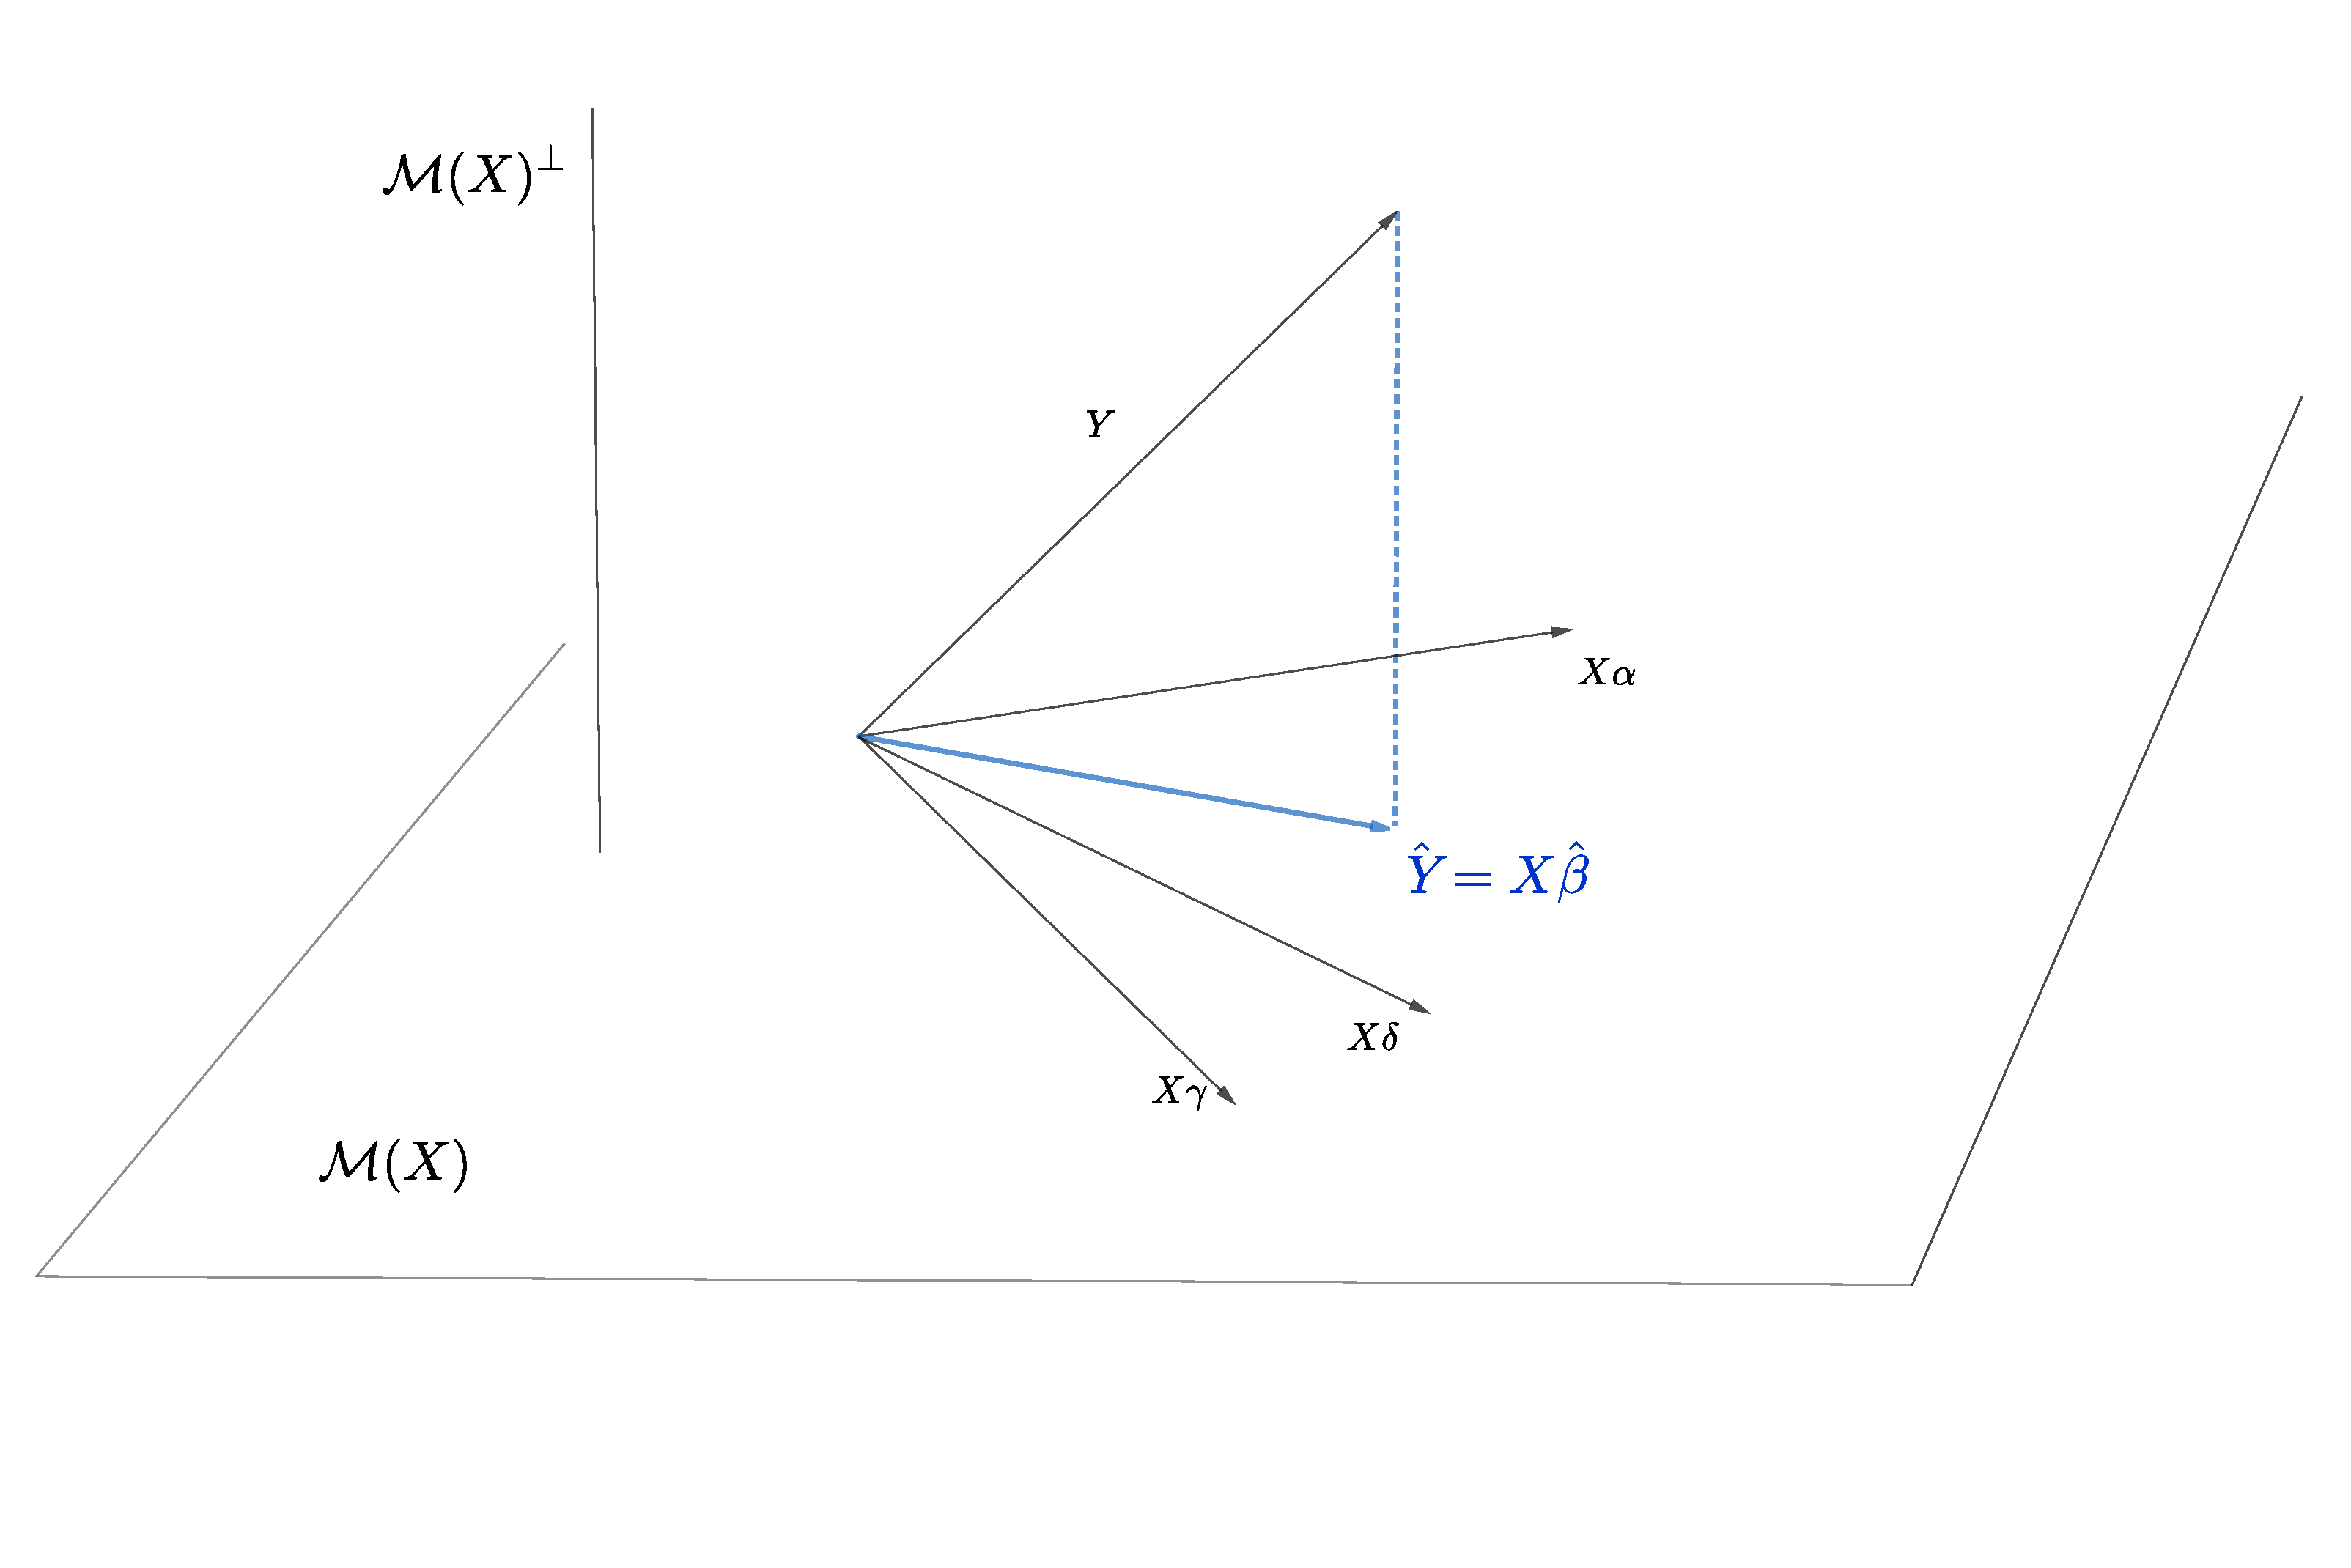
\includegraphics[width=0.8\linewidth]{images/sem2/RegMult_p1} \end{center}

\begin{enumerate}
\def\labelenumi{\alph{enumi})}
\setcounter{enumi}{1}
\tightlist
\item
  Metoda analitică
\end{enumerate}

O a doua metodă este metoda analitică. Problema noastră cere să căutăm
vectorul \(\boldsymbol \beta\in\mathbb{R}^{p+1}\) care minimizează
funcția

\begin{align*}
S(\boldsymbol \beta) &= \left\lVert \boldsymbol Y - \boldsymbol X \boldsymbol\beta\right\rVert^2 = \left(\boldsymbol Y - \boldsymbol X \boldsymbol\beta\right)^\intercal\left(\boldsymbol Y - \boldsymbol X \boldsymbol\beta\right) = \boldsymbol Y^\intercal \boldsymbol Y - \boldsymbol Y^\intercal \boldsymbol X \boldsymbol\beta - \boldsymbol \beta^\intercal \boldsymbol X^\intercal \boldsymbol Y + \boldsymbol \beta^\intercal \boldsymbol X^\intercal \boldsymbol X \boldsymbol\beta \\
  & = \boldsymbol \beta^\intercal \boldsymbol X^\intercal \boldsymbol X \boldsymbol\beta - 2 \boldsymbol Y^\intercal \boldsymbol X \boldsymbol\beta + \lVert  \boldsymbol Y \rVert^2
\end{align*}

unde am folosit faptul că
\(\boldsymbol Y^\intercal \boldsymbol X \boldsymbol\beta = \left(\boldsymbol Y^\intercal \boldsymbol X \boldsymbol\beta\right)^\intercal = \boldsymbol \beta^\intercal \boldsymbol X^\intercal \boldsymbol Y\)
(sunt elemente de dimensiune \(1\times 1\)). Pentru aceasta trebuie să
rezolvăm ecuația \(\nabla S(\boldsymbol \beta) = 0\) și să verificăm că
soluția este într-adevăr punct de minim.

Reamintim că dacă \(f:\mathbb{R}^k\to\mathbb{R}\) atunci

\[
\nabla f = \frac{\partial f}{\partial \boldsymbol x^\intercal} = \begin{pmatrix}\frac{\partial f}{\partial x_1} & \frac{\partial f}{\partial x_2} & \cdots & \frac{\partial f}{\partial x_k}\end{pmatrix}.
\]

În particular, pentru
\(f(\boldsymbol x) = \boldsymbol a^\intercal \boldsymbol x\) (formă
liniară) avem

\[
  \nabla f = \frac{\partial \boldsymbol a^\intercal \boldsymbol x}{\partial \boldsymbol x^\intercal} = \begin{pmatrix}\frac{\partial \sum_{i=1}^{k}a_i x_i}{\partial x_1} & \frac{\partial \sum_{i=1}^{k}a_i x_i}{\partial x_2} & \cdots & \frac{\partial \sum_{i=1}^{k}a_i x_i}{\partial x_k}\end{pmatrix} = \boldsymbol a^\intercal
\]

iar
\(\frac{\partial \boldsymbol a^\intercal \boldsymbol x}{\partial \boldsymbol x} = \boldsymbol a\).

În cazul în care \(f\) este o aplicație liniară,
\(f(\boldsymbol x) = A \boldsymbol x\) unde
\(A\in\mathcal{M}_{m,k}(\mathbb{R})\), atunci

\[
  A \boldsymbol x = \begin{pmatrix}\sum_{j=1}^{k}a_{1j} x_j\\
  \sum_{j=1}^{k}a_{2j} x_j\\
  \vdots\\
  \sum_{j=1}^{k}a_{mj} x_j\end{pmatrix}, \qquad \frac{\partial A \boldsymbol x}{\partial x_j} = \begin{pmatrix}a_{1j}\\
  a_{2j}\\
  \vdots\\
  a_{mj}\end{pmatrix}
\]

și

\[
  \frac{\partial A \boldsymbol x}{\partial \boldsymbol x^\intercal} = \begin{pmatrix}\begin{pmatrix}a_{11}\\
  a_{21}\\
  \vdots\\
  a_{m1}\end{pmatrix}, \ldots, \begin{pmatrix}a_{1j}\\
  a_{2j}\\
  \vdots\\
  a_{mj}\end{pmatrix}, \ldots, \begin{pmatrix}a_{1k}\\
  a_{2k}\\
  \vdots\\
  a_{mk}\end{pmatrix}\end{pmatrix} = \begin{pmatrix}a_{11} & \cdots & a_{1j} & \cdots & a_{1k}\\
  \vdots & \ddots & \vdots & \ddots & \vdots\\
  a_{i1} & \cdots & a_{ij} & \cdots & a_{ik}\\
  \vdots & \ddots & \vdots & \ddots & \vdots\\
  a_{m1} & \cdots & a_{mj} & \cdots & a_{mk}
  \end{pmatrix} = A.
\]

În mod similar se poate verifica și relația
\(\frac{\partial \boldsymbol x^\intercal A^\intercal}{\partial \boldsymbol x} = A^\intercal\).

Dacă \(f\) este o formă pătratică
\(f(\boldsymbol x) = \boldsymbol x^\intercal A \boldsymbol x\) cu
\(A\in\mathcal{M}_{k}(\mathbb{R})\) (matrice pătratică de ordin \(k\)),
atunci

\[
  \boldsymbol x^\intercal  A \boldsymbol x = \sum_{i = 1}^{k}\sum_{j = 1}^{k}a_{ij}x_ix_j = \sum_{i = 1}^{k}a_{ii}x_i^2 + \sum_{i = 1}^{k}\sum_{\substack{j = 1\\ j\neq i}}^{k}a_{ij}x_ix_j 
\]

de unde

\[
  \frac{\partial \boldsymbol x^\intercal  A \boldsymbol x}{\partial x_r} = 2 a_{rr}x_r + \sum_{j\neq r}a_{rj}x_j + \sum_{i\neq r}a_{ir}x_i = \sum_{j = 1}^{k}a_{rj}x_j + \sum_{i = 1}^{k}a_{ir}x_i
\]

prin urmare

\[
  \frac{\partial \boldsymbol x^\intercal  A \boldsymbol x}{\partial \boldsymbol x} = \begin{pmatrix}\frac{\partial \boldsymbol x^\intercal  A \boldsymbol x}{\partial x_1}\\
  \vdots\\
  \frac{\partial \boldsymbol x^\intercal  A \boldsymbol x}{\partial x_k}\end{pmatrix} = \begin{pmatrix}\sum_{j = 1}^{k}a_{1j}x_j + \sum_{i = 1}^{k}a_{i1}x_i\\
  \vdots\\
  \sum_{j = 1}^{k}a_{kj}x_j + \sum_{i = 1}^{k}a_{ik}x_i\end{pmatrix} = A\boldsymbol x + A^\intercal \boldsymbol x.
\]

De asemenea putem observa că
\(\frac{\partial \boldsymbol x^\intercal A \boldsymbol x}{\partial \boldsymbol x^\intercal} = \left(A\boldsymbol x + A^\intercal \boldsymbol x\right)^\intercal = \boldsymbol x^\intercal A^\intercal + \boldsymbol x^\intercal A\).

În plus, dacă \(A\in\mathcal{M}_{k}(\mathbb{R})\) este o matrice
simetrică (\(A^\intercal = A\)) atunci

\[
  \frac{\partial \boldsymbol x^\intercal  A \boldsymbol x}{\partial \boldsymbol x} = 2A\boldsymbol x, \quad \frac{\partial \boldsymbol x^\intercal  A \boldsymbol x}{\partial \boldsymbol x^\intercal} = 2\boldsymbol x^\intercal A^\intercal.
\]

Revenind la problema noastră observăm că \(S(\boldsymbol \beta)\) este
pătratică în \(\boldsymbol \beta\) iar matricea
\(\boldsymbol X^\intercal \boldsymbol X\) este simetrică, prin urmare

\[
\nabla S(\boldsymbol \beta) = \frac{\partial S(\boldsymbol \beta)}{\partial \boldsymbol \beta^\intercal} = \frac{\partial }{\partial \boldsymbol \beta^\intercal}\left(\boldsymbol \beta^\intercal \boldsymbol X^\intercal \boldsymbol X \boldsymbol\beta - 2 \boldsymbol Y^\intercal \boldsymbol X \boldsymbol\beta + \lVert  \boldsymbol Y \rVert^2\right) = 2 \boldsymbol \beta^\intercal (\boldsymbol X^\intercal \boldsymbol X)  - 2 \boldsymbol Y^\intercal \boldsymbol X = 0 
\]

este echivalentă cu \emph{sistem de ecuații normale} (prin trecerea la
transpusă)

\[
(\boldsymbol X^\intercal \boldsymbol X)\boldsymbol \beta = \boldsymbol X^\intercal\boldsymbol Y
\]

care atunci când ipoteza \(\mathcal{H}_1\) este adevărată, ceea ce
conduce la inversabilitatea matricei
\(\boldsymbol X^\intercal \boldsymbol X\) (are valori proprii nenule),
revine la

\[
\hat{\boldsymbol \beta} = (\boldsymbol X^\intercal \boldsymbol X)^{-1} \boldsymbol X^\intercal \boldsymbol Y.
\]

Pentru a arăta că \(\hat{\boldsymbol \beta}\) este într-adevăr un punct
de minim pentru \(S(\boldsymbol \beta)\) trebuie să arătăm că matricea
hessiană este pozitiv definită. Matricea hessiană, ținând cont de
simetria matricii \(\boldsymbol X^\intercal \boldsymbol X\), este

\[
  \frac{\partial^2 S(\boldsymbol \beta)}{\partial \boldsymbol \beta\partial \boldsymbol \beta^\intercal} = \frac{\partial}{\partial \boldsymbol \beta}\left(\frac{\partial S(\boldsymbol \beta)}{\partial \boldsymbol \beta^\intercal}\right) = \frac{\partial}{\partial \boldsymbol \beta}\left(2 \boldsymbol \beta^\intercal (\boldsymbol X^\intercal \boldsymbol X)  - 2 \boldsymbol Y^\intercal \boldsymbol X\right) =  2 \boldsymbol X^\intercal \boldsymbol X
\]

iar pentru \(\boldsymbol u\in\mathbb{R}^{p+1}\backslash\{0\}\) avem

\[
  \boldsymbol u^\intercal \frac{\partial^2 S(\boldsymbol \beta)}{\partial \boldsymbol \beta\partial \boldsymbol \beta^\intercal} \boldsymbol u = \boldsymbol u^\intercal \left(2 \boldsymbol X^\intercal \boldsymbol X\right) \boldsymbol u  = \langle \boldsymbol X\boldsymbol u, \boldsymbol X\boldsymbol u\rangle = 2\lVert \boldsymbol X\boldsymbol u\rVert^2 > 0
\] deci \(\boldsymbol X^\intercal \boldsymbol X\) este pozitiv definită
prin urmare și
\(\frac{\partial^2 S(\boldsymbol \beta)}{\partial \boldsymbol \beta\partial \boldsymbol \beta^\intercal}\)
este pozitiv definită.

\subsection{Interpretări geometrice}\label{interpretari-geometrice-1}

\begin{center}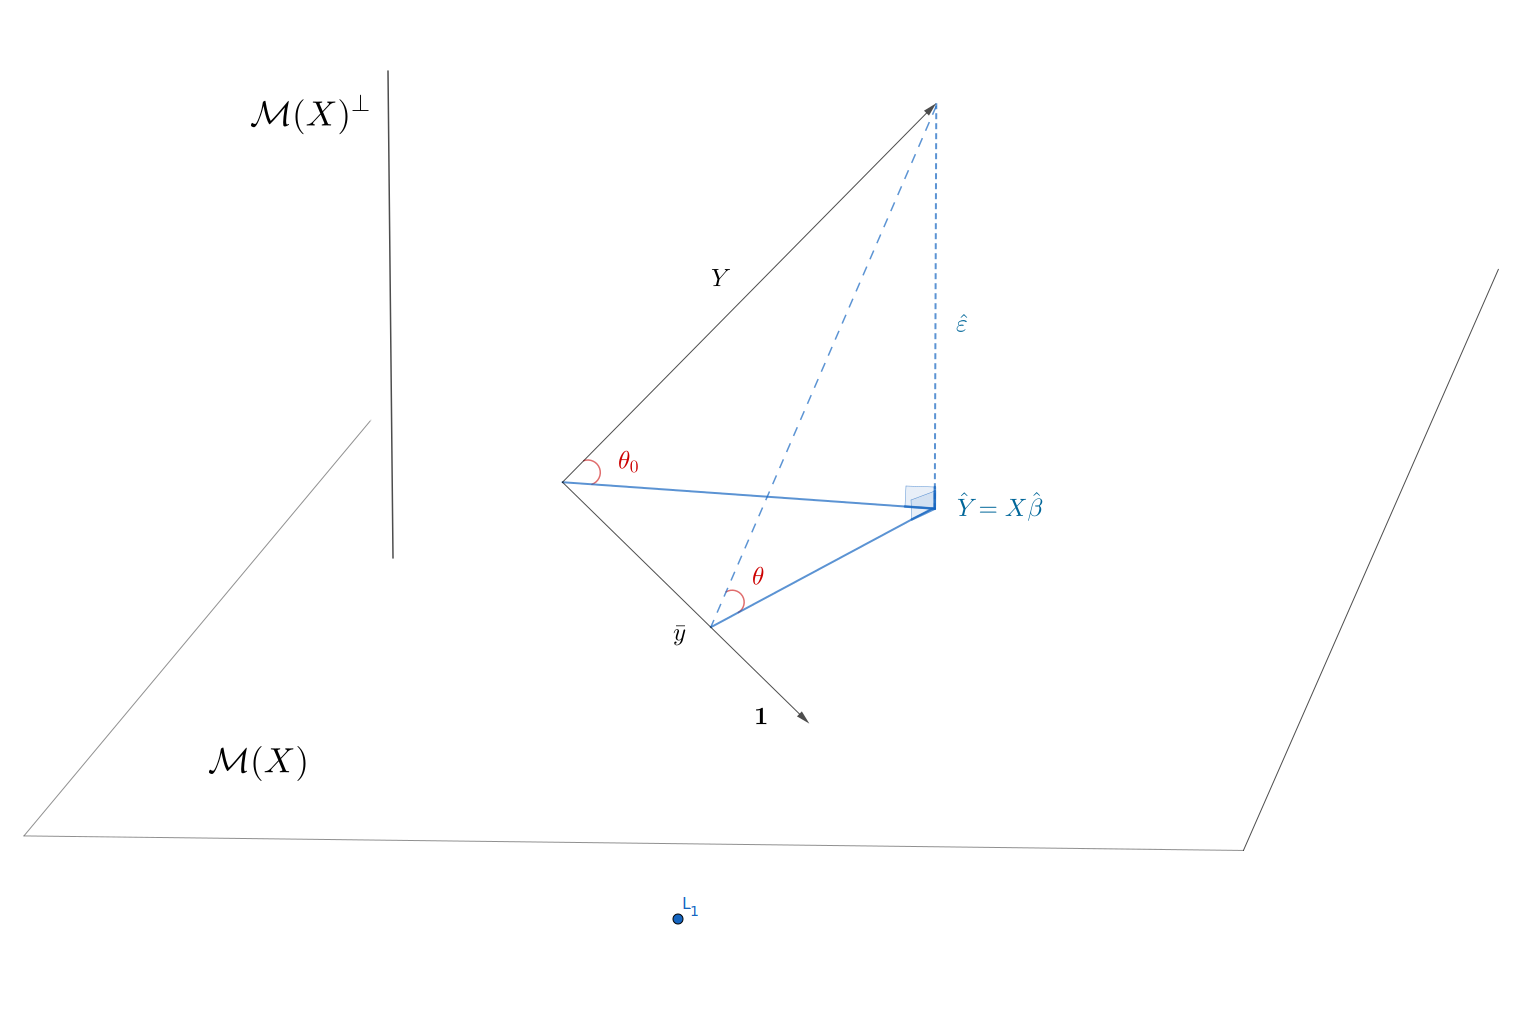
\includegraphics[width=0.8\linewidth]{images/sem2/RegMult_p2} \end{center}

\subsection{Modelul condiționat
normal}\label{modelul-conditionat-normal}

\bibliography{references/InstStatFin2018ref.bib}


\end{document}
